\chapter{Sekilas Tentang Aplikasi Prediksi}

\section{Apa itu Prediksi ?}
\par Prediksi adalah suatu proses memperkirakan secara sistematis tentang sesuatu yang paling mungkin terjadi di masa depan berdasarkan informasi masa lalu dan sekarang yang dimiliki, agar kesalahannya (selisih antara sesuatu yang terjadi dengan hasil perkiraan) dapat diperkecil. Prediksi tidak harus memberikan jawaban secara pasti kejadian yang akan terjadi, melainkan berusaha untuk mencari jawaban sedekat mung\\ kin yang akan terjadi (Herdianto, 2013 : 8) .\\

\par Pengertian Prediksi sama dengan ramalan atau perkiraan. Menurut kamus besar bahasa Indonesia, prediksi adalah hasil dari kegiatan memprediksi atau meramal atau memperkirakan nilai pada masa yang akan datang dengan menggunakan data masa lalu. Prediksi menunjukkan apa yang akan terjadi pada suatu keadaan tertentu dan merupakan input bagi proses perencanaan dan pengambilan keputusan.\\

\par Prediksi bisa berdasarkan metode ilmiah ataupun subjektif belaka. Ambil contoh, prediksi cuaca selalu berdasarkan data dan informasi terbaru yang didasarkan pengamatan termasuk oleh satelit. Begitupun prediksi gempa, gunung meletus ataupun bencana secara umum. Namun, prediksi seperti pertandingan sepakbola, olahraga, dll umumnya berdasarkan pandangan subjektif dengan sudut pandang sendiri yang memprediksinya. \\

\par Permulaan awal, walaupun pengkajian yang mendalam mengenai alternatif masa depan adalah suatu disiplin baru, barangkali orang telah menaruh perhatian besar tentang apa yang akan terjadi kemudian semenjak manusia mulai mengetahui sesuatu. Populasi tukang ramal dan tukang nujum pada zaman kuno dan abad pertengahan merupakan satu manifestasi dari keinginan tahu orang tentang masa depannya. Perhatian tentang masa depan ini berlangsung terus bahkan berkembang menjadi kolom astrologi yang disindikatkan pada tahun 1973. \\

\par Secara Eksplisit, pembahasan mengenai teori peramalan kebijakan sangatlah sedikit. Namun, secara implisit, peramalan kebijakan terkait menjadi satu dengan proses analisa kebijakan. Karena didalam menganalisa kebijakan, untuk menformulasikan sebuah rekomendasi kebijakan baru, maka diperlukan adanya peramalan-peramalan atau prediksi mengenai kebijakan yang akan diberlakukan dimasa yang akan datang. Namun, satu dari sekian banyak prosedur yang ditawarkan oleh para pakar Dunn, masih memberikan pembahasan tersendiri mengenai peramalan kebijakan. Menurut Dunn, Peramalan Kebijakan ( policy forecasting) merupakan suatu prosedur untuk membuat informasi factual tentangsituasi social masa depan atas dasar informasi yang telah ada tentang masalah kebijakan.\\

\par Peramalan (forecasting) adalah suatu prosedur untuk membuat informasi factual tentang situasi sosial masa depan atas dasar informasi yang telah ada tentang masalah kebijakan. Ramalan mempunyai tiga bentuk utama: proyeksi, prediksi, dan perkiraan. 
\begin{enumerate}
\item Suatu proyeksi adalah ramalan yang didasarkan pada ekstrapolasi atas kecenderungan masa lalu maupun masa kini ke masa depan. Proyeksi membuat pertanyaan yang tegas berdasarkan argument yang diperoleh dari motode tertentu dan kasus yang paralel.
\item Sebuah prediksi adalah ramalan yang didasarkan pada asumsi teoritik yang tegas. Asumsi ini dapat berbentuk hokum teoretis (misalnya hokum berkurangnya nilai uang), proposisi teoritis (misalnya proposisi bahwa pecahnya masyarakat sipil diakibatkan oleh kesenjangan antara harapan dan kemampuan), atau analogi (misalnya analogi antara pertumbuhan organisasi pemerintah dengan pertumbuhan organisme biologis).
\item Suatu perkiraan (conjecture) adalah ramalan yang didasarkan pada penilaian yang informative atau penilaian pakar tentang situasi masyarakat masa depan.\\
\end{enumerate}

\par Tujuan dari pada diadakannya peramalan kebijakan adalah untuk memperoleh informasi mengenai perubahan dimasa yang akan dating yang akan mempengaruhi terhadap implementasi kebijakan serta konsekuensinya. Oleh karenanya, sebelum rekomendasi diformulasikan perlu adanya peramalan kebijakan sehingga akan diperoleh hasil rekomendasi yang benar-benar akurat untuk diberlakukan pada masa yang akan. Didalam memprediksi kebutuhan yang akan datang dengan berpijak pada masa lalu, dibutuhkan seseorang yang memiliki daya sensitifitas tinggi dan mampu membaca kemungkinan-kemungkinan dimasa yang akan datang. Permalan kebijakan juga diperlukan untuk mengontrol, dalam artian, berusaha merencanakan dan menetapkan kebijakan sehingga dapat memberikan alternatif-alternatif tindakan yang terbaik yang dapat dipilih diantara berbagai kemungkinan yang ditawarkan oleh masa depan. Masa depan juga terkadang banyak dipengaruhi oleh masa lalu. Dengan mengacu pada masa depan analisis kebijakan harus mampu menaksir nilai apa yang bisa atau harus membimbing tindakan di masa depan.\\



\section{Tujuan \textit{Prototype}}
Prototipe bertujuan untuk contoh atau model awal yang dibangun untuk menguji sebuah konsep atau proses atau aksi sebagai sesuatu yang digandakan atau dipelajarinya. Pengertian prototipe tidak selalu merujuk pada ukuran, artinya prototipe tidak selalu harus berukuran sama dengan produk yang akan dibuat. Prototipe bisa berukuran lebih kecil atau lebih besar dibanding dengan produk yang akan dibuat asalkan aksi atau proses yang akan terjadi sebenarnya . 

Prototype dapat memberikan ide bagi pembuat dan pemakai potensial tentang cara sistem berfungsi dalam bentuk lengkapnya. Tujuannya adalah mengembangkan model menjadi sistem final. Artinya sistem akan dikembangkan lebih cepat daripada metode tradisional dan biayanya menjadi lebih murah. Selain hal tersebut pembuatan prototipe untuk perbaikan atau penyempurnaan rancangan .

\section{Bahasa Pemograman C}
\subsection{Sejarah Bahasa C}
Bahasa C merupakan perkembangan dari bahasa BCPL yang dikembangkan oleh Martin Richards pada tahun 1967. Selanjutnya bahasa ini memberikan ide kepada Ken Thompson yang kemudian mengembangkan bahasa yang disebut bahasa B pada tahun 1970. Perkembangan selanjutnya dari bahasa B adalah bahasa C oleh Dennis Ricthie sekitar tahun 1970-an di Bell Telephone Laboratories Inc. (sekarang adalah AT&T Bell Laboratories). Bahasa C pertama kali digunakan di computer Digital Equipment Corporation PDP-11 yang menggunakan system operasi UNIX. Hingga saat ini penggunaan bahasa C telah merata di seluruh dunia. Hampir semua perguruan tinggi di dunia menjadikan bahasa C sebagai salah satu mata kuliah wajib. Selain itu, banyak bahasa pemrograman populer seperti PHP dan Java menggunakan sintaks dasar yang mirip bahasa C. Oleh karena itu, kita juga sangat perlu mempelajarinya .
    
\subsection{Pengertian Bahasa Pemograman C}
C merupakan perkembangan dari bahasa pemrograman c yang di ciptakan oleh Brian W. Kerninghan dan Dennis M. Ritchie lalu di kembangkan oleh Bjarne Stroustrup dari Laboratorium Bell, AT&T, pada tahun 1983. C cukup kompatibel dengan bahasa pendahulunya C. Pada mulanya C disebut “ a better C “. Nama C sendiri diberikan oleh Rick Mascitti pada tahun 1983, yang berasal dari operator increment pada bahasa C. Keistimewaan yang sangat berari dari C ini adalah karena bahasa ini mendukung Pemrograman Berorientasi Objek (OOP /Object Oriented Programming) .

Bahasa pemograman C ini dapat digunakan untuk memprogram sebuah robot, Untuk memprogram menggunakan bahasa C ini dapat menggunakan IDE \textit{ (Integrated Development Environment)} salah satu contonya yaitu IDE Arduino. 

\subsection{Kelebihan dan Kekurangan Bahasa C}
Dalam bahasa pemograman C ini memiliki  kelebihan yaitu sebagai berikut :
\begin{enumerate}
\item Bahasa C tersedia hampir di semua jenis computer. 
\item Kode bahasa C sifatnya adalah portable dan fleksibel untuk semua jenis computer. 
\item Bahasa C hanya menyediakan sedikit kata-kata kunci, hanya terdapat 32 kata kunci.
\item Proses executable program bahasa C lebih cepat 
\item Dukungan pustaka yang banyak.
\item C adalah bahasa yang terstruktur 
\item Bahasa C termasuk bahasa tingkat menengah

\end{enumerate}

Selain memiliki kelebihan bahasa pemograman C juga mempunyai kekurangannya yaitu :
\begin{enumerate}
    \item Banyaknya Operator serta fleksibilitas penulisan program kadang-kadang membingungkan pemakai. 
    \item Bagi pemula pada umumnya akan kesulitan menggunakan pointer.
\end{enumerate}

\section{Penggunaan Bahasa C menggunakan Arduino IDE}
\subsection{Arduino IDE}
Arduino IDE \textit{(Integrated Development Environment)} adalah software yang di gunakan untuk memprogram di arduino, dengan kata lain Arduino IDE sebagai media untuk memprogram board Arduino. Arduino IDE bisa di download secara gratis di website resmi Arduino IDE.

Arduino IDE ini berguna sebagai text editor  untuk membuat,  mengedit, dan juga mevalidasi kode program. bisa juga digunakan untuk meng-upload ke board Arduino.  Kode program yang digunakan pada Arduino disebut dengan istilah Arduino “sketch”  atau disebut juga source code arduino, dengan ekstensi file source code .ino

Arduino IDE dibuat dari bahasa pemrograman JAVA. Arduino IDE juga dilengkapi dengan library C/C++ yang biasa disebut Wiring yang membuat operasi input dan output menjadi lebih mudah. Arduino IDE ini dikembangkan dari software Processing yang dirombak menjadi Arduino IDE khusus untuk pemrograman dengan Arduino.

Dalam \textit{Softwere} Arduino IDE ini dapat memprogram kode tidak hanya \textit{microcontroller} arduino saja, tetapi pada \textit{softwere} ini dapat digunakan untuk memprogram \textit{microcontroller} yang lain salah satu contohnya yaitu Nodemcu.

\subsection{Bagian-Bagian Arduino IDE}

\begin{figure}[H]
\centering
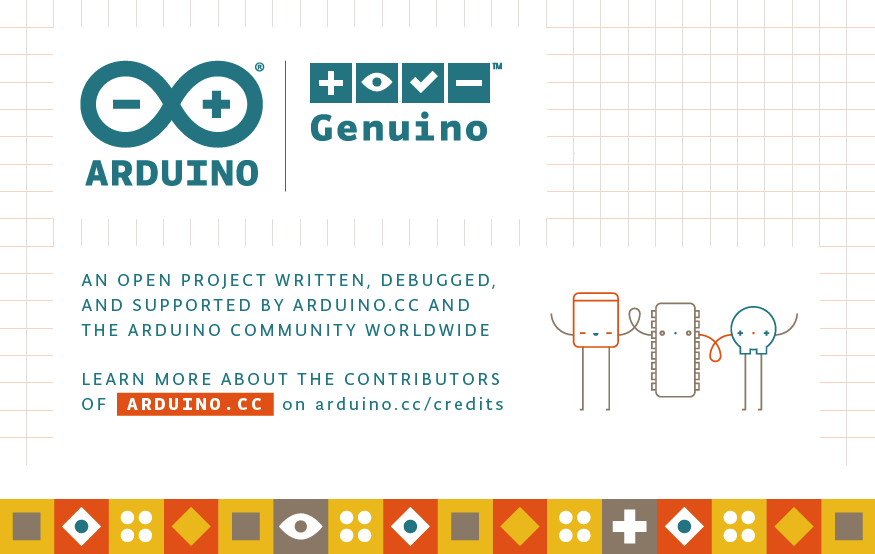
\includegraphics[width=1\textwidth]{figures/ide.png}
\caption{Arduino IDE}
\label{print}
\end{figure}
Editor \textit{Programming} pada umumnya memiliki fitur untuk \textit{cut / paste} dan untuk \textit{find / replace teks}, demikian juga pada Arduino IDE. Pada bagian keterangan aplikasi memberikan pesan balik saat menyimpan dan mengekspor serta sebagai tempat menampilkan kesalahan. Konsol log menampilkan teks log dari aktifitas Arduino IDE, termasuk pesan kesalahan yang lengkap dan informasi lainnya. Pojok kanan bawah menampilkan \textit{port} serial yang di gunakan. Tombol \textit{toolbar} terdapat ikon tombol pintas untuk memverifikasi dan meng-upload program, membuat, membuka, dan menyimpan \textit{sketch}, dan membuka monitor serial. Untuk lebih jelasnya perhatikan gambar dibawah ini :

\begin{figure}[H]
\centering
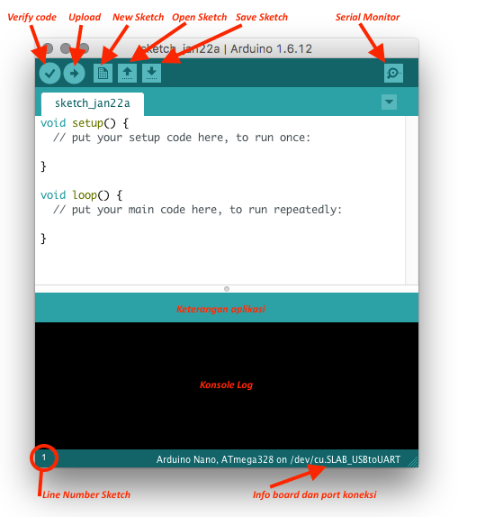
\includegraphics[width=1\textwidth]{figures/arduino.png}
\caption{Tampilan Arduino IDE}
\label{print}
\end{figure}

\begin{enumerate}
    \item \textbf{Verify} pada versi sebelumnya dikenal dengan istilah Compile. Sebelum aplikasi di-upload ke board Arduino, biasakan untuk memverifikasi terlebih dahulu sketch yang dibuat. Jika ada kesalahan pada sketch, nanti akan muncul error. Proses Verify / Compile mengubah sketch ke binary code untuk di-upload ke mikrokontroller.
    \item \textbf{Upload} tombol ini berfungsi untuk mengupload sketch ke board Arduino. Walaupun kita tidak mengklik tombol verify, maka sketch akan di-compile, kemudian langsung diupload ke board. Berbeda dengan tombol verify yang hanya berfungsi untuk memverifikasi source code saja.
    \item \textbf{New Sketch} Membuka window dan membuat sketch baru
    \item \textbf{Open Sketch} Membuka sketch yang sudah pernah dibuat. Sketch yang dibuat dengan IDE Arduino akan disimpan dengan ekstensi file .ino
    \item \textbf{Save Sketch}menyimpan sketch, tapi tidak disertai dengan mengkompile.
    \item \textbf{Serial Monitor} Membuka interface untuk komunikasi serial, nanti akan kita diskusikan lebih lanjut pada bagian selanjutnya.
    \item \textbf{Keterangan Aplikasi} pesan-pesan yang dilakukan aplikasi akan muncul di sini, misal \textit{Compiling} dan \textit{Done Uploading} ketika kita \textit{mengcompile} dan mengupload sketch ke board Arduino
    \item \textbf{Konsol log} Pesan-pesan yang dikerjakan aplikasi dan pesan-pesan tentang sketch akan muncul pada bagian ini. Misal, ketika aplikasi mengcompile atau ketika ada kesalahan pada sketch yang kita buat, maka informasi error dan baris akan diinformasikan di bagian ini.
    \item \textbf{Baris Sketch} bagian ini akan menunjukkan posisi baris kursor yang sedang aktif pada sketch.
    \item \textbf{nformasi Board dan Port} Bagian ini menginformasikan port yang dipakai oleh board Arduino.
\end{enumerate}


\subsection{\textit{Sketch} Arduino}
\par Pada arduino bahasa pemrograman yang digunakan adalah bahasa C/C++. Program pada Arduino terbagi menjadi tiga bagian utama yaitu Structure, Values (berisi variable dan konstantata) dan yang terakhir function. Struktur kode pada arduino yaitu berisi fungsi  setup() dan loop() sebagai berikut :
\begin{enumerate}
 \item \textbf{Setup()}
   \par  fungsi ini dipanggil pertama kali ketika menjalankan \textit{sketch}. digunakan sebagai tempat \textit{inisialisai variable, pin mode}, penggunaan \textit{library} dan lainnya. fungsi ini dijalankan sekali ketika \textit{board} dinyalakan atau di \textit{reset} . Berikut contoh dari void setup :
    \begin{figure}
        \centering
        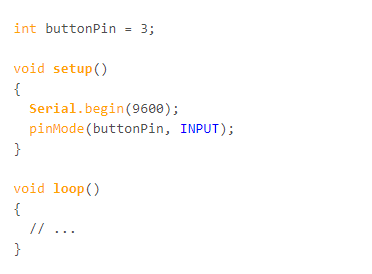
\includegraphics[width=1\textwidth]{figures/setup.png}
        \caption{Contoh Void Setup}
        \label{print}
    \end{figure}
    
    \item \textbf{loop()}
    \par Setelah membuat fungsi setup() sebagai tempat \textit{inisialisai variabel} dan menetapkan nilai maka selanjutnya fungsi loop() seperti namanya fungsi ini akan melakukan perulangan berturu-turut, memungkina program untuk mengubah dan menanggapi. digunakan untuk mengontrol \textit{board} Arduino. Berikut contoh dari void loop :
   

\begin{figure}[H]
\centering
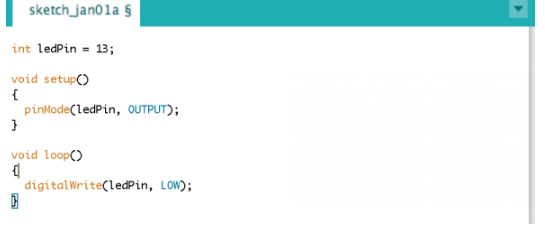
\includegraphics[width=1\textwidth]{figures/contoh.png}
\caption{Gambar Contoh Fungsi Setup dan Loop}
\label{print}
\end{figure}

\par Pada gambar 2.4 merupakan suatu contoh fungsi void setup dan void loop pada pemograman bahasa C menggunakan Arduino IDE.

\item \textbf{Values}
\par Berisi variable atau konstanta sesuai dengan type data yang didukung oleh Arduino.
\item \textbf{Function}
\par Segmentasi kode ke fungsi memungkinkan programmer untuk membuat potongan-potongan modular kode yang melakukan tugas yang terdefinisi dan kemudian kembali ke asal kode dari mana fungsi itu “dipanggil”. Umumnya menggunakan fungsi adalah ketika salah satu kebutuhan untuk melakukan tindakan yang sama beberapa kali dalam sebuah program.
\item \textbf{Tipe Data Pada Arduino}
\par Tipe data merupakan kelompok data berdasarkan jenis-jenis tertentu. Tipe data banyak dijumpai dalam berbagai bahasa pemrograman. Begitu juga dalam pemrograman Arduino. Tipe-tipe data yang digunakan dalam pemrograman Arduino antara lain adalah Void, Boolean, Char, Unsigned Char, Byte, Int, Unsigned Int, Word, Long, Unsigned Long, Short, Float, dan Double.
\begin{enumerate}
    \item \textbf{Void}
    \par Kata kunci void digunakan dalam deklarasi fungsi. Kata kunci ini menandakan bahwa fungsi tersebut tidak mengembalikan informasi ke fungsi yang dipanggil. Seperti sourcode dibawah ini :
     \lstinputlisting{src/void.c}
     
    \item \textbf{Boolean}
    \par Boolean menangani satu dari dua nilai yaitu, benar (true) atau salah (false). Setiap variabel Boolean menempati satu byte memori. Seperti sourcode dibawah ini :
     \lstinputlisting{src/boolean.c}
     \item\textbf{Char}
     \par Tipe data Char adalah tipe data yang mengambil satu byte memori yang menyimpan suatu nilai karakter. Karakter harfiah ditulis dalam kutip tunggal, misalnya ‘A’ dan untuk multi karakter digunakan tanda kutip ganda, seperti “ABC”.

    \par Namun demikian, karakter-karakter tersebut disimpan sebagai angka. Hal ini dapat dilihat dengan jelas pada Tabel ASCII. Hal ini berarti bahwa  melakukan operasi aritmatika pada karakter, di mana nilai karakter ASCII digunakan. Sebagai contoh, ‘A’ + 1 memiliki nilai 66, karena nilai ASCII dari huruf kapital A adalah 65.
    \lstinputlisting{src/char.c}
    \item \textbf{Unsigned char}
    \par Unsigned char merupakan tipe data tak bertanda yang mencakup satu byte memori. Tipe data ini meng-encode bilangan dari 0 sampai 255.
    \lstinputlisting{src/unchar.c}
    
    \item \textbf{Byte}
    \par Byte menyimpan bilangan tak bertanda 8 bit, dari 0 sampai 255.
    \lstinputlisting{src/byte.c}
    \item \textbf{INT}
    \par Integer adalah tipe data utama untuk penyimpanan bilangan. int menyimpan nilai 16-bit (2-byte). Rentang nilanya adalah kisaran -32.768 hingga 32.767 
    \par Ukuran int berbeda-beda setiap papan arduino. Sebagai contoh untuk Arduino Due, int menyimpan nilai 32-bit (4-byte). Rentang nilainya dari -2,147,483,648 sampai 2,147,483,647.
    \lstinputlisting{src/int.c}
    \item\textbf{Unsigned int}
    \par Unsigned int sama dengan int dalam cara mereka menyimpan nilai 2 byte. Unsigned int hanya menyimpan nilai positif, menghasilkan rentang dari 0 hingga 65.535. Arduino Due menyimpan nilai 4 byte (32-bit), mulai dari 0 hingga 4.294.967.295.
    \lstinputlisting{src/unint.c}
    \item \textbf{Long}
    \par Variabel dengan tipe Long merupakan penyimpanan bilangan dengan ukuran diperluas, dan menyimpan 32 bit (4 byte), dari -2,147,483,648 sampai 2,147,483,647.
    \lstinputlisting{src/long.c}
    
    \item \textbf{Unsigned long}
    \par Unsigned Long merupakan tipe Long tak bertanda yang diperluas untuk penyimpanan bilangan dan menyimpan 32 bit (4 byte). Tidak seperti long standar, unsigned long tidak akan menyimpan angka negatif, rentangnya dari 0 hingga 4.294.967.295.
    \lstinputlisting{src/unlong.c}
    
    \item \textbf{Short}
    \par Shot adalah tipe data 16-bit. Pada semua Arduino (berbasis ATMega dan ARM), short menyimpan nilai 16-bit (2-byte). Rentang nilainya antara 32.768 hingga 32.767.
    \lstinputlisting{src/short.c}
    
    \item \textbf{Float}
    \par Tipe data untuk bilangan floating-point adalah bilangan yang memiliki titik desimal. Angka floating-point sering digunakan untuk memperkirakan nilai analog dan kontinu karena memiliki resolusi lebih besar daripada bilangan bulat.

    \par Bilangan floating-point dapat memiliki nilai maksimal 3,4028235E + 38 dan nilai minimal -3,4028235E + 38. Float disimpan sebagai informasi 32 bit (4 byte).
    \lstinputlisting{src/float.c}
    
    \item \textbf{Double}
    \par Pada Arduino Uno dan arduino berbasis ATMEGA lainnya, bilangan floating-point presisi ganda menempati empat byte. Artinya, implementasi ganda persis sama dengan float, tanpa perolehan presisi. Pada Arduino Due, ganda memiliki presisi 8-byte (64 bit).

    \lstinputlisting{src/double.c}
\end{enumerate}
\item \textbf{Variabel}
\par Variabel dalam bahasa pemrograman C, dimana bahasa C ini digunakan dalam Arduino, memiliki suati properti yang disebut dengan cakupan \textit{(scope)}. Suatu cakupan merupakan wilayah dari program dan ada tiga tempat dimana variabel dapat dideklarasikan. Ketiga tempat tersebut adalah sebagai berikut :
\begin{enumerate}
    \item Di dalam fungsi atau blok, variabel ini disebut dengan variabel lokal \textit{(local variable).}
    \item Di dalam definisi parameter fungsi, yang disebut dengan parameter formal \textit{(formal parameters).}
    \item Di luar semua fungsi, variabel ini disebut dengan variabel global \textit{(global variable).}
\end{enumerate}
\item \textbf{Variabel Local \textit{ (Local Variable)}}
\par Sebagaimana disebutkan di atas, bahwa variabel lokal merupakan variabel yang dideklarasikan di dalam suatu fungsi atau blok. Variabel lokal ini hanya dapat digunakan oleh pernyataan (statement) yang berada di dalam fungsi atau blok kode. Berikut ini adalah contoh penggunaan dari variabel lokal.
\lstinputlisting{src/variabel1.c}

\item \textbf{Variabel Global \textit{(Global Variable)}}
\par Variabel global \textit{(Global variable)}didefinisikan di luar seua dungsi, biasanya pada bagian atas dari program. Variabel global akan menyimpan nilainya sepanjang program dijalankan \textit{ (life-time).}
\lstinputlisting{src/variabel2.c}

\par Variabel global dapat diakses oleh semua fungsi apapun. Artinya variabel global akan tersedia terus untuk digunakan di seluruh program setelah dideklarasikan.Berikut ini adalah contoh penggunaan dari variabel global dalam pemrograman Arduino.


\end{enumerate}

\section{Komponen yang Digunakan Untuk Pembuatan \textit{Prototype} PKA}
Komponen yang digunakan untuk membuat sebuah \textit{prototype} prediksi ketinggian air (PKA) untuk pendeteksi banjir peringatan dini yaitu sebagai berikut :
\begin{enumerate}
    \item \textbf{NodeMCU}
   \par  NodeMCU adalah ESP8266 (khususnya seri ESP-12, termasuk ESP-12E) maka fitur – fitur yang dimiliki NodeMCU akan kurang lebih sama ESP-12 (juga ESP-12E untuk NodeMCU v.2 dan v.3) kecuali NodeMCU telah dibungkus oleh API sendiri yang dibangun berdasarkan bahasa pemrograman eLua, yang kurang lebih cukup mirip dengan javascript. Selain dapat diprogram menggunakan bahasa LUA dapat juga diprogram menggunakan bahasa C menggunakan arduino IDE. Beberapa fitur didalamnya antara lain : 
    \begin{enumerate}
        \item 0 Port GPIO dari D0 – D10
        \item Fungsionalitas PWM
        \item Antar muka I2C dan SPI
        \item Antar muka 1 Wire
        \item ADC
    \end{enumerate}
\par NodeMCU pada dasarnya pengembangan dari ESP 8266
dengan firmware berbasis e-Lua. Pada NodeMcu dilengkapi dengan micro usb port yang berfungsi untuk pemorgaman maupun power supply. Selain itu juga pada NodeMCU di lengkapi dengan tombol push button yaitu tombol reset dan flash. NodeMCU menggunakan bahasa pemorgamanan Lua yang merupakan package dari esp8266. Bahasa Lua memiliki logika dan susunan pemorgaman yang sama dengan c hanya berbeda syntax. Jika menggunakan bahasa Lua maka dapat menggunakan tool Lua loader maupun Lua uploder.
\par Selain dengan bahasa Lua NodeMCU juga support dengan sofware
Arduino IDE dengan melakukan sedikit perubahan board manager pada
Arduino IDE.
\par Sebelum digunakan Board ini harus di Flash terlebih dahulu agar support terhadap tool yang akan digunakan. Jika menggunakan Arduino IDE menggunakan firmware yang cocok yaitu firmware keluaran dari AiThinker yang support AT Command. Untuk penggunaan tool loader Firmware yang di gunakan adalah firmware NodeMCU.
    
\begin{figure}[H]
\centering
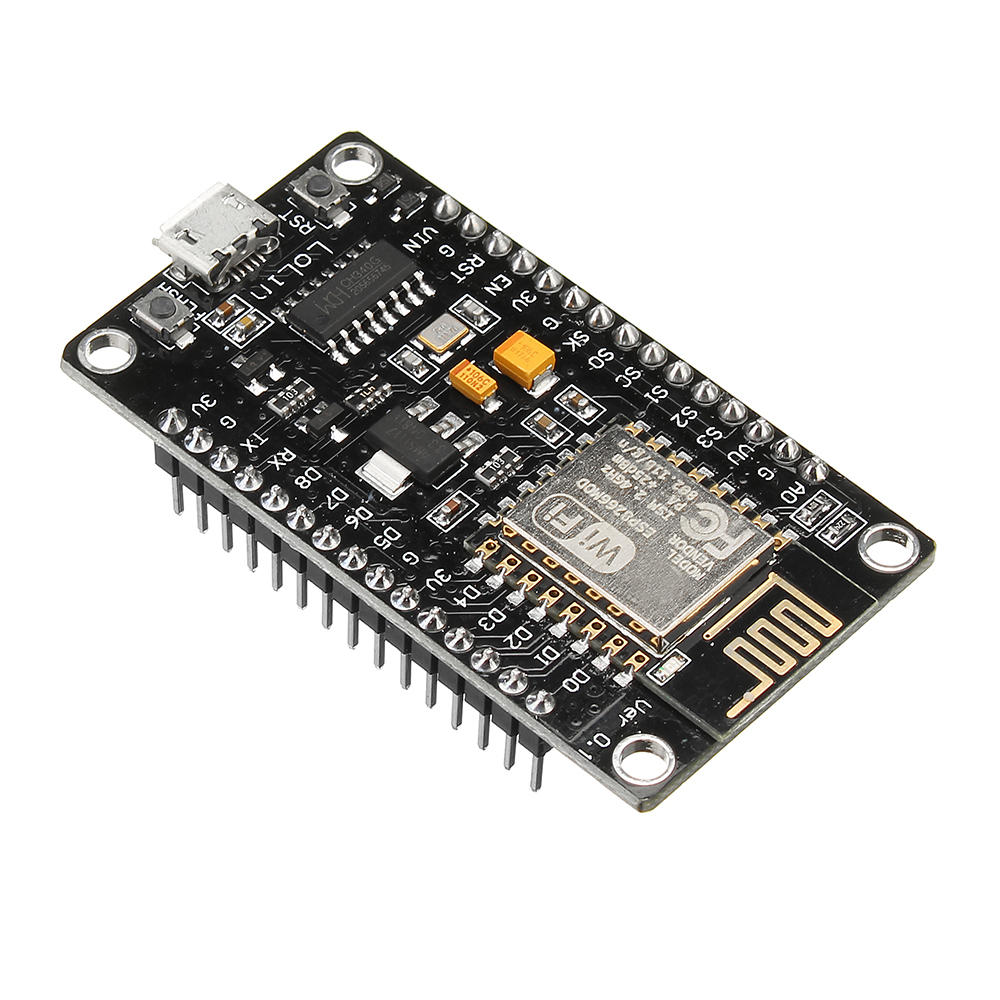
\includegraphics[width=1\textwidth]{figures/node.jpg}
\caption{NodeMCU}
\label{print}
\end{figure}

\par Pada gambar 2.5 merupakan sebuah NodeMCU yang akan digunakan sebagai \textit{microcontroller} untuk pembuatan \textit{prototype} prediksi ketinggian air (PKA) untuk pendeteksi banjir peringatan dini dengan notifikasi melalui bot telegram .
\item \textbf{Spesifikasi \textit{Datasheet} NodeMCU}
\begin{figure}[H]
\centering
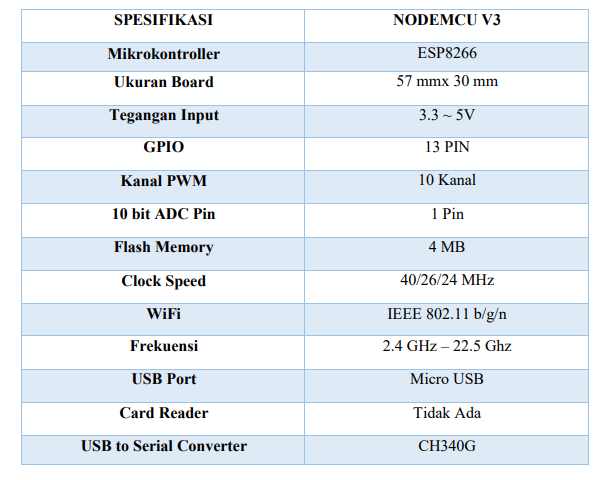
\includegraphics[width=1\textwidth]{figures/spesifikasi.png}
\caption{Spesifikasi NodeMCU}
\label{print}
\end{figure}

\begin{figure}[H]
\centering
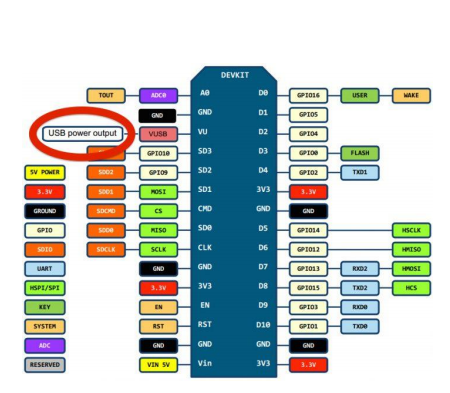
\includegraphics[width=1\textwidth]{figures/skemanode.png}
\caption{Skema Posisi Pin NodeMCU}
\label{print}
\end{figure}

\item \textbf{\textit{Protokol Hypertext Transfer Protoco} (HTTP)}
\par \textit{Hypertext Transfer Protocol} (HTTP) adalah sebuah protokol jaringan lapisan aplikasi yang digunakan untuk sistem informasi terdistribusi, kolaboratif, dan menggunakan hipermedia.

\par Protokol HTTP didefinisikan oleh Tim Berners-Lee dalam RFC
1945 versi 1.0 dan digunakan sejak tahun 1990. Penyempurnaan protokol HTTP menjadi versi 1.1 yang dispesifikasikan oleh IETF dengan RFC 2616. HTTP bersifat \textit{request – response}, yaitu HTTP \textit{client}(\textit{user} agen misalnya) mengirimkan permintaan \textit{(request)} ke HTTP server dan server merespon sesuai request tersebut. User agen sebagai contoh adalah Mozilla,Netscape,Google Chrome, atau browser berbasis teks contohnya Lynx atau links dan sebagainya. 
\par Pada protokol HTTP terdapat 3 jenis hubungan dengan perantara
proxy, gateway, dan tunnel. Proxy bertindak sebagai agent penerus,
menerima request dalam bentuk Uniform Resource Identifier (URI) absolut,mengubah format request dan mengirimkan request ke server yang ditunjukan oleh URI. 4 Gateway bertindak sebagai agen penerima dan menterjemahkan request ke protokol server yang dilayaninya. Tunnel bertindak sebagai titik Relay antara dua hubungan HTTP tanpa mengubah request dan response HTTP. Tunnel digunakan jika komunikasi perlu melalui sebuah perantara dan perantara tersebut tidak mengetahui isi pesan dalam hubungan tersebut. 
\par Perbedaan mendasar antara HTTP/1.1 dengan HTTP/1.0 adalah
penggunaan hubungan persistent. HTTP/1.0 membuka satu koneksi untuk tiap permintaan satu URI, sedangkan HTTP/1.1 dapat menggunakan sebuah koneksi TCP untuk beberapa permintaan URI (persistent) \textit{(header Conection : keepAlive)}, kecuali jika \textit{client} menyatakan tidak hendak menggunakan hubungan \textit{persistent (header Conection : close)} . HTTP \textit{port} TCP default adalah 80, namun itu bisa diganti dengan nomor TCP lain diantara 1023 – 65535.

\item \textbf{Sensor Ultrasonic HC-SR04}
\par Sensor jarak ultrasonic HC-SR04 adalah sensor 40 KHz. HC-SR04 merupakan sensor ultrasonik yang dapat digunakan untuk mengukur jarak antara penghalang dan sensor. Konfigurasi pin dan tampilan sensor HC-SR04 diperlihatkan pada gambar dibawah :
\begin{figure}[H]
\centering
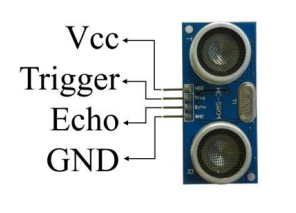
\includegraphics[width=1\textwidth]{figures/sensor2.png}
\caption{Sensor HC-SR04}
\label{print}
\end{figure}

\par HC-SR04 memiliki 2 komponen utama sebagai penyusunnya yaitu ultrasonic transmitter dan ultrasonic receiver. Fungsi dari ultrasonic transmitter adalah memancarkan gelombang ultrasonik dengan frekuensi 40 KHz kemudian ultrasonic receiver menangkap hasil pantulan gelombang ultrasonik yang mengenai suatu objek. Waktu tempuh gelombang ultrasonik dari pemancar hingga sampai ke penerima sebanding dengan 2 kali jarak antara sensor dan bidang
pantul seperti yang diperlihatkan pada gambar :
\begin{figure}[H]
\centering
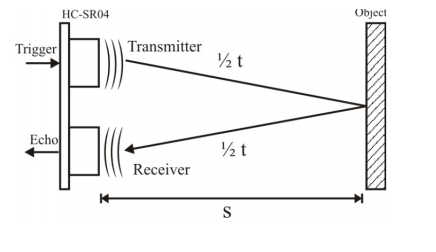
\includegraphics[width=1\textwidth]{figures/sr04.png}
\caption{Prinsip Pengukuran Jarak Sensor HC SR04}
\label{print}
\end{figure}
\par Prinsip pengukuran jarak menggunakan sensor ultrasonik HC-SR04 adalah, ketika pulsa trigger diberikan pada sensor, transmitter akan mulai memancarkan gelombang ultrasonik, pada saat yang sama sensor akan menghasilkan output TTL transisi naik menandakan sensor mulai menghitung waktu pengukuran, setelah receiver menerima pantulan yang dihasilkan oleh suatu objek maka pengukuran waktu akan dihentikan dengan menghasilkan output TTL transisi turun. Jika waktu pengukuran adalah t dan kecepatan suara adalah 340 m/s, maka jarak antara sensor dengan objek dapat dihitung dengan menggunakan Persamaan berikut :
\begin{figure}[H]
\centering
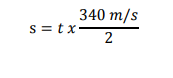
\includegraphics[width=1\textwidth]{figures/rumus2.png}
\caption{Rumus Perhitungan Jarak}
\label{print}
\end{figure}

Spesifikasi Sensor HC-SR04 :
\begin{enumerate}
    \item Tegangan Kerja: DC 5V
    \item \textit{Operating Current}: 15mA
    \item Frekuensi Kerja: 40Hz
    \item Jarak Pengukuran Maks: 4m
    \item Jarak Pengukuran Mins: 2cm
    \item Mengukur Sudut: 15 derajat
    \item Sinyal Input Pemicu: 10μS TTL pulsa
    \item inyal Output Echo Input sinyal tuas TTL dan kisaran proporsionals
    \item Dimensi 45 * 20 * 15mm
\end{enumerate}

\begin{figure}[H]
\centering
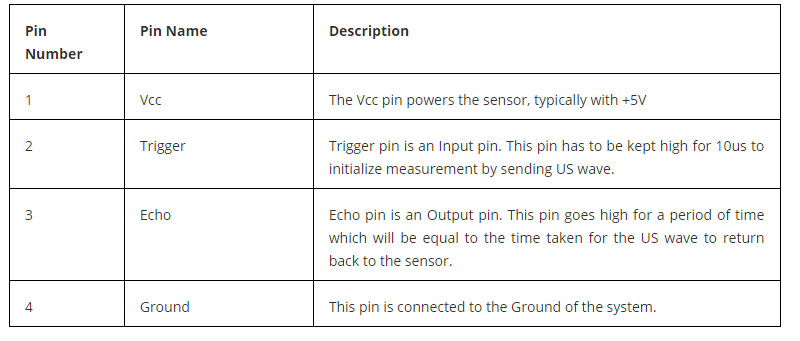
\includegraphics[width=1\textwidth]{figures/konfig.png}
\caption{Konfigurasi Sensor Ultrasonic HC-SR04}
\label{print}
\end{figure}

\par HC-SR04 mempunyai  modul rentang ultrasonik yang menyediakan fungsi pengukuran non-kontak 2 cm hingga 400 cm. Akurasi mulai dapat mencapai 3mm dan sudut efektif adalah <15 °. Itu dapat didukung dari catu daya 5V.

\par Power Sensor menggunakan + 5V melalui Vcc pin Ground dari sensor. Saat Sensor kurang dari 15mA dan karenanya dapat langsung didukung oleh papan 5V pin (Jika tersedia). Trigger dan pin Echo keduanya / O pin dan karenanya mereka dapat terhubung ke I / pin O dari mikrokontroler. Untuk memulai pengukuran, pemicu pin harus dibuat tinggi untuk 10us dan kemudian dimatikan. Tindakan ini akan memicu gelombang ultrasonik pada frekuensi 40Hz dari pemancar dan penerima akan menunggu untuk gelombang untuk kembali. Setelah gelombang dikembalikan setelah dipantulkan oleh objek apa pun, pin Echo menjadi tinggi untuk jumlah waktu tertentu yang akan sama dengan waktu yang dibutuhkan gelombang untuk kembali ke sensor.


\item \textbf{Sensor Ultrasonic  US 100}

\par Sensor US-100 adalah versi peningkatan dari US-020 Ultrasonic Sensor pada kelasnya HC-SR04 memiliki performa lebih bagus dibanding US-020) yang sudah dilengkapi dengan fitur kompensasi temperatur. Di kelasnya \textit{(ultrasonic range sensor with temperature compensation)} US-100 merupakan modul sensor jarak terbaik.
\par Modul jarak ultrasonik bekerja dengan sistem sonar seperti yang digunakan pada kapal selam, yaitu dengan melepaskan sinyal dalam bentuk gelombang ultrasonik (gelombang suara dengan frekuensi sangat tinggi di luar jangkauan pendengaran telinga manusia) dan mengukur waktu hingga gelombang tersebut dipantulkan. Dengan mengetahui kecepatan suara di udara, kita dapat mengubah besaran waktu ini menjadi jarak dengan rumus:\\ jarak = ( selisih waktu * kecepatan suara d iudara ) / 2.
\par Fitur kompensasi suhu ini sangatlah penting untuk meningkatkan akurasi sensor sejenis ini berhubung kecepatan rambat suara di udara sangat terpengaruh oleh suhu / temperatur. Suara adalah sejenis energi kinetis. Molekul pada suhu tinggi memiliki tingkat energi lebih tinggi yang membuat mereka bergetar (vibrate) lebih cepat. Karena molekul ini bergetar lebih cepat, gelombang suara yang melewatinya dapat merambat dengan kecepatan lebih tinggi. Kecepatan rambat suara di udara pada suhu ruang (25°C) sekitar 346 meter per detik, sementara pada suhu beku (0°C), kecepatannya menurun menjadi 331 meter per detik. Untuk setiap derajat celcius kenaikan suhu, kecepatan rambatannya bertambah 60 cm per detik.
\par \textit{Distance }Sensor US-100 ini mengukur suhu lingkungan (ambience temperature) dengan sensor suhu terpadu sehingga dapat mengkompensasi perbedaan suhu, menghasilkan pengukuran jarak yang sangat akurat. Berikut Gambar Sensor US 100 :
\begin{figure}[H]
\centering
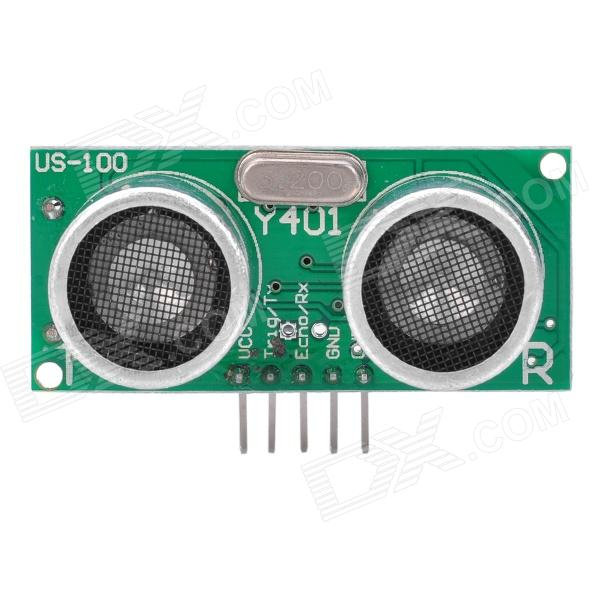
\includegraphics[width=0.5\textwidth]{figures/sensor.jpg}
\caption{Gambar Sensor Ultrasonic US 100}
\label{print}
\end{figure}

\par Sensor ultrasonic menggunakan daya + 5V yang diatur melalui pin Vcc ad Ground dari sensor. Arus yang dikonsumsi oleh sensor kurang dari 15mA dan karenanya dapat langsung ditenagai oleh pin 5V on board (Jika tersedia). Trigger dan Echo pin keduanya adalah pin I / O dan karenanya mereka dapat dihubungkan ke pin I / O dari mikrokontroler. Untuk memulai pengukuran, pin pemicu harus dibuat tinggi untuk 10uS dan kemudian dimatikan. Tindakan ini akan memicu gelombang ultrasonik pada frekuensi 40Hz dari pemancar dan penerima akan menunggu gelombang kembali. Setelah gelombang dikembalikan setelah dipantulkan oleh objek apa pun, pin Echo menjadi tinggi untuk jumlah waktu tertentu yang akan sama dengan waktu yang dibutuhkan gelombang untuk kembali ke sensor . 

\par Jumlah waktu selama pin Echo tetap tinggi diukur oleh MCU / MPU karena memberikan informasi tentang waktu yang dibutuhkan untuk gelombang untuk kembali ke Sensor.

\item \textbf{Prinsip kerja Sensor ultrasonic}
\begin{figure}[H]
\centering
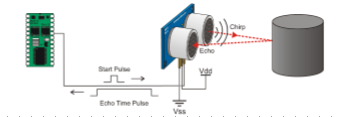
\includegraphics[width=1\textwidth]{figures/kerja.png}
\caption{Prinsip Kerja Sensor Ultrasonic}
\label{print}
\end{figure}

\par Seperti yang ditunjukkan di atas, sensor adalah modul 4 pin, yang pin namanya masing-masing adalah Vcc, Trigger, Echo dan Ground. Sensor ini adalah sensor yang sangat populer digunakan dalam banyak aplikasi di mana mengukur jarak atau objek penginderaan diperlukan. Modul sensor Ultrasonik adalah cara mudah untuk mengukur jarak dari benda. Modul ini memiliki banyak aplikasi seperti sensor parkir, hambatan dan sistem pemantauan medan, pengukuran jarak industri, dll. Sistem ini memiliki stabilitas kinerja dan akurasi tinggi mulai dari 2cm hingga 450cm.Modul ini memiliki dua mata seperti proyek di bagian depan yang membentuk pemancar dan Penerima Ultrasonik. Sensornya bekerja dengan rumus :

\begin{figure}[H]
\centering
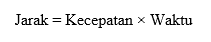
\includegraphics[width=1\textwidth]{figures/rumus.png}
\caption{Rumus perhitungan Jarak Sensor Ultrasonic}
\label{print}
\end{figure}

\par Pemancar ultrasonik mentransmisikan gelombang ultrasonik, gelombang ini bergerak di udara dan ketika ia keberatan dengan bahan apa pun itu dipantulkan kembali ke sensor gelombang. Untuk menghitung jarak menggunakan rumus di atas, harus mengetahui kecepatan dan waktu. Karena menggunakan gelombang Ultrasonik, kecepatan universal gelombang AS pada kondisi ruangan yang 330m / s. Sirkuit inbuilt pada modul akan menghitung waktu yang dibutuhkan untuk gelombang US untuk kembali dan menyalakan pin gema tinggi untuk jumlah waktu yang sama, dengan cara ini kita juga dapat mengetahui waktu yang dibutuhkan. Sekarang cukup hitung jaraknya menggunakan mikrokontroler atau mikroprosesor.

\item  \textbf{Spesifikasi(\textit{DataSheet})Sensor Ultrasonik US 100}\\
Spesifikasi atau \textit{Datasheet} dari sensor ultrasonic US 100 sebagai berikut :\\
\begin{enumerate}
    \item Tegangan input: 5V DC
    \item \textit{Quiescent current}: kurang dari 2mA
    \item output: 5V tinggi
    \item Level output: pada akhir 0V
    \item Sudut induksi: tidak lebih dari 15 derajat
    \item Jarak deteksi: 2cm-450cm
    \item Presisi: hingga 1mm
    \item Dimensi: 4.4cm x 2.6cm x 1.4cm
    \item Berat: 43g
\end{enumerate}
Adapun pin konfigurasi dari sensor ultrasonic Us 100 yaitu :
\begin{figure}[H]
\centering
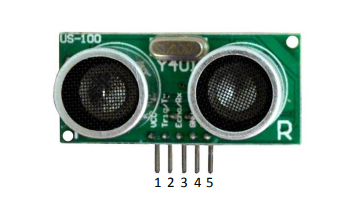
\includegraphics[width=1\textwidth]{figures/us.png}
\caption{Pin Konfigurasi}
\label{print}
\end{figure}

\begin{enumerate}
    \item VCC: 5V DC
    \item Trig: trigger input
    \item Echo: pulse output
    \item GND: ground
    \item GND: ground
\end{enumerate}

Skema diagram sensor ultrasonic US 100 yaitu :
\begin{figure}[H]
\centering
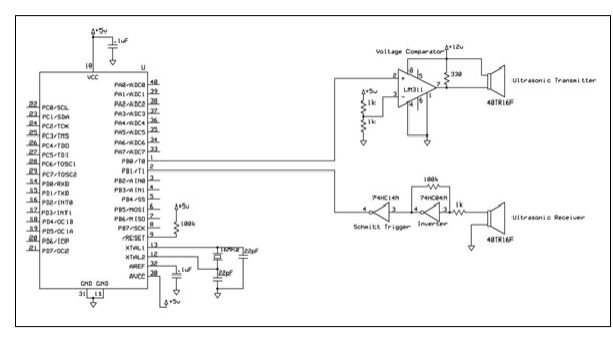
\includegraphics[width=1\textwidth]{figures/skema.png}
\caption{Skema diagram sensor ultrasonic US 100}
\label{print}
\end{figure}
\item Cara \textbf{\textit{Test Sensor Ultrasonic US 100}}\\
Komponen yang akan digunakan adalah:
\begin{enumerate}
    \item Mikrokontroler (arduino yang kompatibel)
    \item Modul sensor Ultrasonik US-100 
    \item Konektor pin 
    \item readboard Menggunakan kabel USB, sambungkan porta dari mikrokontroler ke komputer.
    \item Kabel USB
\end{enumerate}
Setelah hal diatas sudah terpenuhi maka ikuti langkah verikut ini :
\begin{enumerate}
    \item Hubungkan komponen menggunakan konektor pin. Pin VCC terhubung ke catu daya 5V, pin GND terhubung ke GND dan pin Trig dan Echo terhubung ke pin I / O digital. Nomor pin akan didasarkan pada kode program yang sebenarnya.
    \item Setelah koneksi perangkat keras, masukkan sketsa sampel ke dalam Arduino IDE.
    \item Menggunakan kabel USB, sambungkan porta dari mikrokontroler ke komputer.
    \item \textit{Upload} program.
    \item Lihat hasilnya di monitor serial.
\end{enumerate}

\item \textbf{Sensor Yang Digunakan}\\
\par Pada pembuatan \textit{prototype} prediksi ketinggian air (PKA) untuk mendeteksi banjir peringatan dini ini mengugunakan sensor ultra sonic US 100. Karena sensor ultrasonic US 100 ini akan membaca jarak lebih akurat dibandingkan dengan sensor ultrasonic HC-SR04.

\par Akan tetapi jika teman-teman ingin mengunakan sensor ultrasonic HC-SR04 tidak ada masalah, karena fungsi dari kedua sensor ini sama yaitu untuk membaca atau mengukur jarak dari suatu benda. Hanya saja jika teman-teman memilih sensor ultrasonic US 100 ini akan mengocek pengeluaran yang lebih besar dibandingkan dengan sensor ultrasonic HC-SR04.

\item \textbf{Buzzer}
\par Buzzer merupakan sebuah komponen elektronika yang masuk dalam keluarga transduser, yang dimana dapat mengubah sinyal listrik menjadi getaran suara. Nama lain dari komponen ini disebut dengan \textit{beeper} .
\begin{figure}[H]
\centering
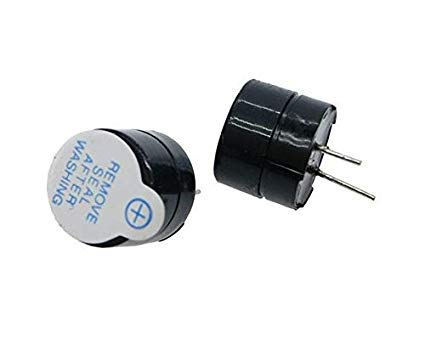
\includegraphics[width=1\textwidth]{figures/buzzer.jpg}
\caption{Buzzer}
\label{print}
\end{figure}

\par Dalam kehidupan sehari – hari, umumnya digunakan untuk rangkaian alarm pada jam, bel rumah, perangkat peringatan bahaya, dan lain sebagainya.Jenis – jenis yang sering ditemukan dipasaran yaitu tipe piezoelectric. Dikarenakan tipe ini memiliki kelebihan seperti harganya yang relatif murah, mudah diaplikasikan ke dalam rangkaian elektronika.

\item \textbf{Cara Kerja Buzzer }
\begin{figure}[H]
\centering
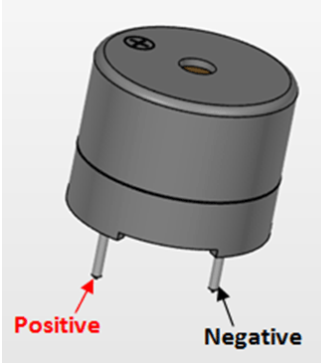
\includegraphics[width=1\textwidth]{figures/buzzer2.png}
\caption{Konfigurasi Pin Buzzer}
\label{print}
\end{figure}
\par Pada saat ada aliran catu daya atau tegangan listrik yang mengalir ke rangkaian yang menggunakan piezoelectric, maka akan terjadi pergerakan mekanis pada piezoelectric tersebut.Yang dimana gerakan tersebut mengubah energi listrik menjadi energi suara yang dapat didengar oleh telinga manusia.Piezoelectric menghasilkan frekuensi di range kisaran antara 1 – 5 kHz hingga 100 kHz yang diaplikasikan ke Ultrasound.Tegangan operasional piezoelectric pada umumnya yaitu berkisar antara 3Vdc hingga 12 Vdc. Adapun konfigurasi pin buzzer yaitu sebagai berikut :

\begin{figure}[H]
\centering
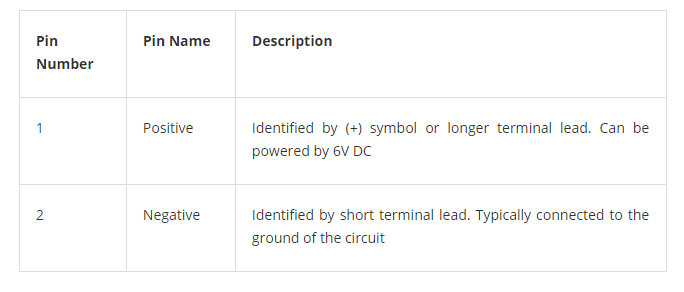
\includegraphics[width=1\textwidth]{figures/buzzer3.png}
\caption{Keterangan Konfigurasi Pin Buzzer}
\label{print}
\end{figure}

\item \textbf{Spesifikasi(\textit{DataSheet)} Buzzer}\\
Spesifikasi atau datasheet dari buzzer meliputi :
\begin{enumerate}
    \item Nilai Tegangan: 6V DC
    \item Tegangan Pengoperasian: 4-8V DC
    \item Nilai \textit{current}: <30mA
    \item Tipe Suara: Bunyi Kontinu
    \item Frekuensi resonansi: ~ 2300 Hz
    \item Kecil dan \textit{package} rapih
\end{enumerate}

\item \textbf{Cara menggunakan Buzzer}\\
\par Buzzer adalah komponen kecil namun efisien untuk menambahkan fitur suara ke proyek / sistem. Ini adalah struktur 2-pin yang sangat kecil dan kompak sehingga dapat dengan mudah digunakan pada Breadboard dan bahkan pada PCB yang menjadikannya komponen yang banyak digunakan dalam sebagian besar aplikasi elektronik.

\par Ada dua jenis buzzers yang umumnya tersedia. Yang ditampilkan di sini adalah buzzer sederhana yang ketika diaktifkan akan membuat suara Continuous Beeepp\\..., jenis lainnya disebut buzzer readymade yang akan terlihat lebih besar daripada ini dan akan menghasilkan Beep. Berbunyi. Berbunyi. Suara karena rangkaian osilasi internal yang ada di dalamnya. Tapi, yang ditunjukkan di sini paling banyak digunakan karena dapat disesuaikan dengan bantuan sirkuit lain agar sesuai dengan mudah dalam \textit{prototype} kita.

\par Buzzer ini dapat digunakan hanya dengan menyalakannya menggunakan catu daya DC mulai dari 4V hingga 9V. Baterai 9V sederhana juga dapat digunakan, tetapi disarankan untuk menggunakan catu daya + 5V atau + 6V yang teregulasi. Buzzer biasanya dikaitkan dengan sirkuit \textit{switching} untuk menghidupkan atau mematikan buzzer pada waktu yang diperlukan dan membutuhkan interval.\\ Adapun diagram buzzer atau model 2D buzzer seperti pada gambar dibawah :

\begin{figure}[H]
    \centering
    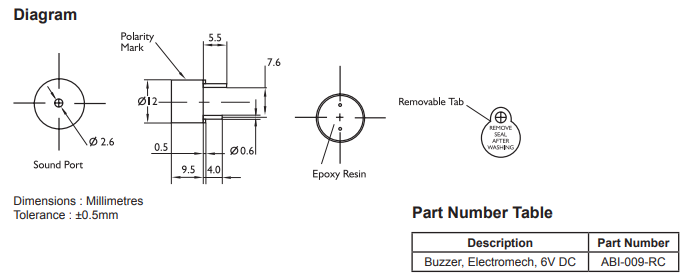
\includegraphics[width=1\textwidth]{figures/buzzer4.png}
    \caption{Diagram model 2D Buzzer}
    \label{print}
\end{figure}

\item \textbf{Led}
\par LED \textit{(Light Emitting Diode)} adalah komponen elektronika yang dapat memancarkan  cahaya monokromatik ketika diberikan tegangan maju. LED merupakan keluarga Dioda yang terbuat dari bahan semikonduktor. Warna-warna Cahaya yang dipancarkan oleh LED tergantung pada jenis bahan semikonduktor yang dipergunakannya. LED juga dapat memancarkan sinar inframerah yang tidak tampak oleh mata seperti yang sering kita jumpai pada Remote Control TV ataupun Remote Control perangkat elektronik lainnya.

\begin{figure}[H]
\centering
\includegraphics[width=0.5\textwidth]{figures/Led.jpg}
\caption{Led}
\label{print}
\end{figure}

\begin{figure}[H]
\centering
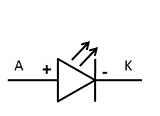
\includegraphics[width=1\textwidth]{figures/simbol.png}
\caption{Simbol Led}
\label{print}
\end{figure}
\par Bentuk LED mirip dengan sebuah bohlam (bola lampu) yang kecil dan dapat dipasangkan dengan mudah ke dalam berbagai perangkat elektronika. Berbeda dengan Lampu Pijar, LED tidak memerlukan pembakaran filamen sehingga tidak menimbulkan panas dalam menghasilkan cahaya.  Oleh karena itu, saat ini LED (Light Emitting Diode) yang bentuknya kecil telah banyak digunakan sebagai lampu penerang dalam LCD TV yang mengganti lampu tube.

\item \textbf{Cara Kerja Led}
\par Seperti dikatakan sebelumnya, LED merupakan keluarga dari Dioda yang terbuat dari Semikonduktor. Cara kerjanya pun hampir sama dengan Dioda yang memiliki dua kutub yaitu kutub Positif (P) dan Kutub Negatif (N). LED hanya akan memancarkan cahaya apabila dialiri tegangan maju (bias forward) dari Anoda menuju ke Katoda.

\par LED terdiri dari sebuah chip semikonduktor yang di doping sehingga menciptakan junction P dan N. Yang dimaksud dengan proses doping dalam semikonduktor adalah proses untuk menambahkan ketidakmurnian (impurity) pada semikonduktor yang murni sehingga menghasilkan karakteristik kelistrikan yang diinginkan. Ketika LED dialiri tegangan maju atau bias forward yaitu dari Anoda (P) menuju ke Katoda (K), Kelebihan Elektron pada N-Type material akan berpindah ke wilayah yang kelebihan Hole (lubang) yaitu wilayah yang bermuatan positif (P-Type material). Saat Elektron berjumpa dengan Hole akan melepaskan photon dan memancarkan cahaya monokromatik (satu warna).

\begin{figure}[H]
\centering
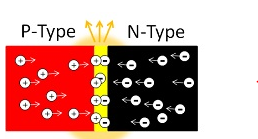
\includegraphics[width=1\textwidth]{figures/kerjaled.png}
\caption{Cara Kerja Led}
\label{print}
\end{figure}

\par LED atau \textit{Light Emitting Diode} yang memancarkan cahaya ketika dialiri tegangan maju ini juga dapat digolongkan sebagai Transduser yang dapat mengubah Energi Listrik menjadi Energi Cahaya.

\item \textbf{Cara Mengetahui Polaritas Led}\\
\begin{figure}[H]
\centering
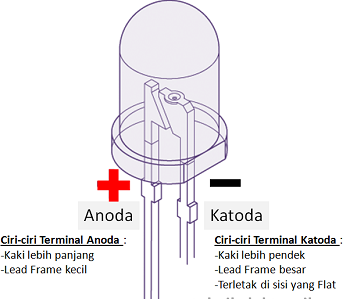
\includegraphics[width=1\textwidth]{figures/polaritas.png}
\caption{Cara Melihat Polaritas}
\label{print}
\end{figure}

\par Untuk mengetahui polaritas terminal Anoda (+) dan Katoda (-) pada LED. Kita dapat melihatnya secara fisik berdasarkan gambar diatas. Ciri-ciri Terminal Anoda pada LED adalah kaki yang lebih panjang dan juga Lead Frame yang lebih kecil. Sedangkan ciri-ciri Terminal Katoda adalah Kaki yang lebih pendek dengan Lead Frame yang besar serta terletak di sisi yang Flat.


\item \textbf{Antares}
\begin{figure}[H]
\centering

\includegraphics[width=1\textwidth]{figures/antares.png}
\caption{Logo Antares}
\label{print}
\end{figure}

\par Antares merupakan sebuah \textit{platform IoT} lokal milik Telkom yang telah mendapat pengakuan dari duna internasional yang dikembangkan oleh departemen media dan digital Telkom MDD. Antares menjadi jembatan dalam solusi IoT yang mendukung berbagai macam protokol yang umum digunakan untuk solusi IoT seperti MQTT, HTTP, websocket, dan CoAP disamping format data JSON dan XML. Selain itu, untuk memudahkan pengembang perangkat lunak dan keras disediakan pula \textit{library} untuk Android dan \textit{microcontroller} berbasia Arduiono.
\begin{figure}[H]
\centering
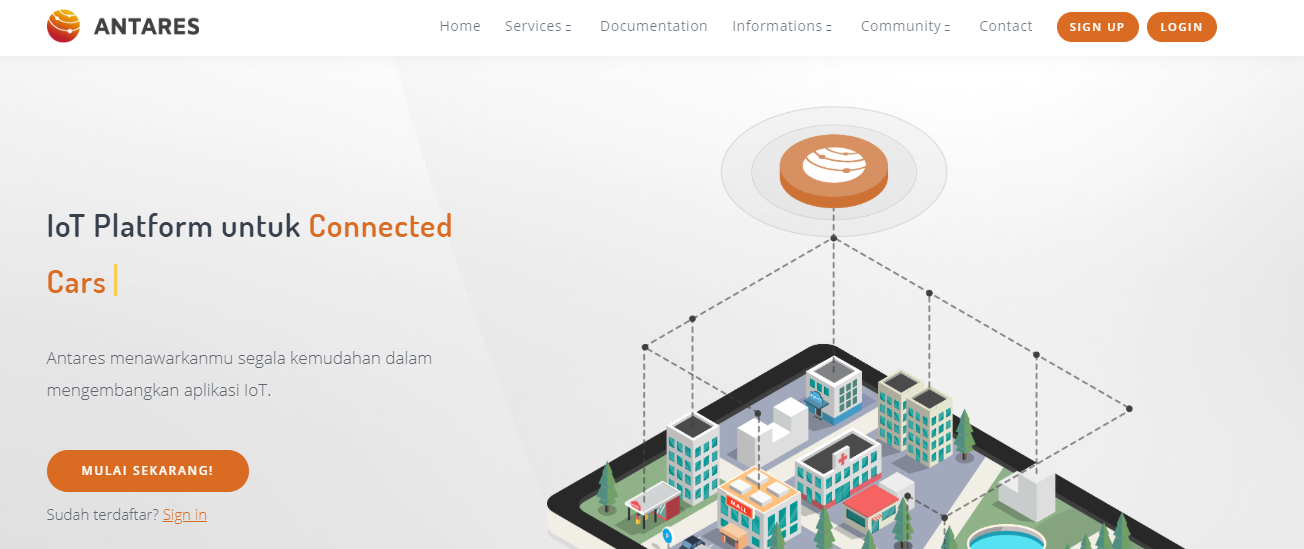
\includegraphics[width=1.1\textwidth]{figures/antares2.png}
\caption{Tampilan Antares Antares}
\label{print}
\end{figure}



\item \textbf{Resistor}
\begin{figure}[H]
\centering
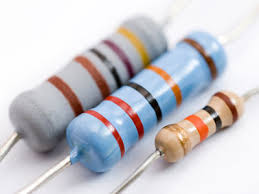
\includegraphics[width=0.7\textwidth]{figures/resistor3.jpg}
\caption{Reistor}
\label{print}
\end{figure}

\par Resistor merupakan komponen elektronika yang tidak memiliki kutub sehingga dapat dipasang bolak balik yang tidak akan menimbulkan masalah pada peralatan elektronika. Pada dasarnya sangat jarang kerusakan barang elektronik disebabkan karena Resistor yang sudah rusak, tetapi jika memang terjadi kerusakan pada resistor tentunya hanya tinggal diganti yang baru dengan ukuran hambatan dan jenis resistor yang sama. Harga resistor di tokoh elektronik sangatlah murah dan untuk mengganti resistor yang rusak di PCB juga sangat mudah.

\par Resistor atau hambatan  salah satu komponen elektronika yang memiliki nilai hambatan tertentu, dimana hambatan ini akan menghambat arus listrik yang mengalir melaluinya. Sebuah resistor biasanya terbuat dari bahan campuran Carbon. Namun tidak sedikit juga resistor yang terbuat dari kawat nikrom, sebuah kawat yang memiliki resistansi yang cukup tinggi dan tahan pada arus kuat. Contoh lain penggunaan kawat nikrom dapat dilihat pada elemen pemanas setrika. Jika elemen pemanas tersebut dibuka, maka terdapat seutas kawat spiral yang biasa disebut dengan kawat nikrom

\par Satuan Resistor adalah Ohm (simbol: Ω) yang merupakan satuan SI untuk resistansi listrik. Dalam sejarah, kata ohm itu diambil dari nama salah seorang fisikawan hebat asal German bernama George Simon Ohm. Beliau juga yang mencetuskan keberadaan hukum ohm yang masih berlaku hingga sekarang.

\item \textbf{Fungsi Resistor}\\
\par Resistor berfungsi sebagai penghambat arus listrik. Jika ditinjau secara mikroskopik, unsur-unsur penyusun resistor memiliki sedikit sekali elektron bebas. Akibatnya pergerakan elektronya menjadi sangat lambat. Sehingga arus yang terukur pada multimeter akan menunjukan angka yang lebih rendah jika dibandingkan rangkaian listrik tanpa resistor.

\par Namun meskipun misalnya kita menyusun rangkaian listrik tanpa resistor, bukan berarti tidak ada hambatan listrik didalamnya. Karena setiap konduktor pasti memiliki nilai hambatan, meskipun relatif kecil. Namun dalam perhitungan matematis, biasanya kita abaikan nilai hambatan pada konduktor tersebut, dan kita anggap konduktor dalam kondisi ideal. Itu berarti besar resistansi konduktor adalah nol.

\item \textbf{Macam-Macam Resistor Sesuai Warna}\\
\begin{figure}[H]
\centering
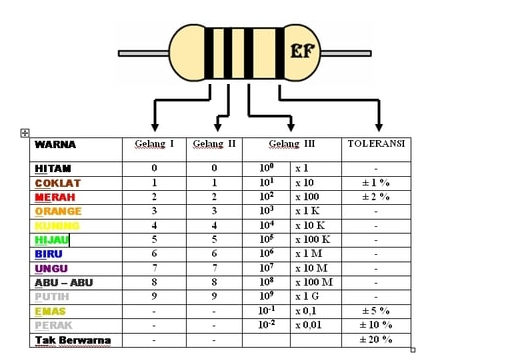
\includegraphics[width=1\textwidth]{figures/resistor2.png}
\caption{Macam-Macam Resistor Sesuai Warna}
\label{print}
\end{figure}

Dari gambar diatas kita dapat menyesuaikan penggunaan resistor untuk kebutuhan kita. 

\item \textbf{Resistor Yang Digunakan}
\par Resistor yang digunakan untuk pembuatan \textit{prototype} prediksi ketinggian air (PKA) untuk mendeteksi banjir peringatan dini ini yaitu resistor 300 OHM 1/2WATT Carbon Film Resistor seperti pada gambar dibawah ini :

\begin{figure}[H]
\centering
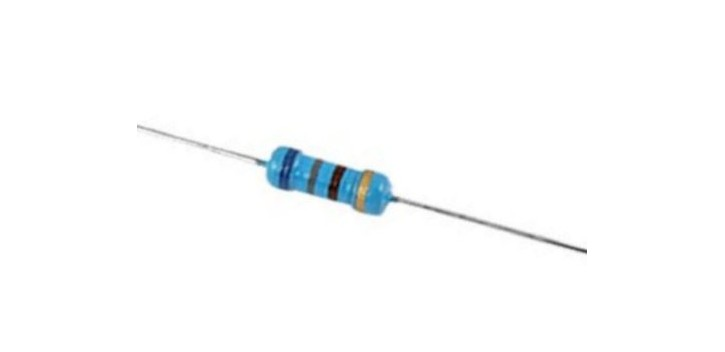
\includegraphics[width=1.3\textwidth]{figures/resistor.jpg}
\caption{Resistor Yang Digunakan}
\label{print}
\end{figure}

\par Resistor 300 OHM 1/2WATT Carbon Film digunakan untuk menjadi hambatan lampu led, agar pada saat lampu led menyala tidak terlalu terang dan tidak menyebabkan sakit mata pada saat dilihat. ResistorResistor 300 OHM 1/2WATT Carbon Film ini cocok digunakan pada prototipe ini karena cocok sebagai hambatan lampu led karena hanya 300 OHM. Sehingga hambatan yang diberikan oleh resistor ini kepada led tidak terlalu besar.
\par Oleh karena itu lampu led akan menyala dengan tingkat penerangan yang sedang tidak terlalu bersinar. Jika kita menggunakan resistor yang hambatannya lebih dari 300 OHM dikhawatirkan lampu led akan menyala sangat redup dikarenakan diberikan hambatan pada lampu led sangat besar. Jika kita memberi hambatan kurang dari 300 OHM pada lampu led .Maka hal yang akan terjadi yaitu lampu led akan memancarkan cahaya sangat terang. Cahaya yang dipancarkan oleh lampu led terlalu terang maka akan mengakibatkan rasa sakit dimata ketika kita melihatnya. Oleh karena itulah kita harus mengetahui hambatan yang diperlukan untuk komponen yang digunakan pada saat membuat project. Selain itu resistor ini akan dipergunakan juga pada buzzer. Sehingga suara yang dikeluarkan oleh buzzer tidak terlalu keras yang dapat merusak indra pendengaran kita. selain itu jika buzzer diberikan hambatan akan mengeluarkan suara yang lebih kecil.

\par Disamping itu harga dari resistor relatif murah. jika kita ingin membeli atau membutuhkan resistor untuk suatu project yang sedang dibuat maupun yang akan dibuat , kalian hanya perlu mengeluarkan biaya \textit{cost} sebanyak Rp.100,- /buah. jika kalian membutuhkan 10 resistor maka kita hanya perlu mengeluarkan Rp.1000,-

\item \textbf{Bot Telegram}
\begin{figure}[H]
\centering

\includegraphics[width=1.4 \textwidth]{figures/telegram.png}
\caption{Logo Telegram}
\label{print}
\end{figure}
\par Seiring Messenger Telegram yang mulai di\textit{install} banyak orang dan dipergunakan untuk percakapan sehari-hari. Memang Telegram belum sepopuler Whatsapp, BBM, maupun Line. Namun, bisa jadi suatu saat akan menjadi suatu messenger yang potensial mendapatkan hati dikalangan masyarakat maya. Menurut Cokrojoyo kelebihan dari Telegram ini adalah adanya landasan untuk mengunakan \textit{Application Programming Interface}(API) untuk masyarakat luas. Salah satu API yang disediakan adalah fitur bot. Bot Telegram adalah bot yang saat ini mulai populer dipergunakan.
\par Keunggulan pertama dari aplikasi Telegram ini adalah fleksibel. Artinya Anda bisa membuat fitur-fitur tambahan yang disertakan dalam aplikasi Telegram ini. Misalkan Anda ingin membuat polling. Anda bisa membuatnya tanpa sendiri dan menambahkan di Telegram Anda tanpa harus menunggu ada update fitur dari Developernya. Sehingga ini membuat Telegram menjadi lebih lebih fleksibel jika dibanding aplikasi sejenis seperti WhatsApp ataupun LineMessenger. Selain itu Keunggulan ke dua dari Telegram adalah pesan berbasis awan (cloud-based message). Artinya dengan Telegram Anda bisa berkomunikasi dengan siapapun (yang juga punya akun Telegram) tanpa batasan device/ gadget.

\item \textbf{Akrilik}
\begin{figure}[H]
\centering
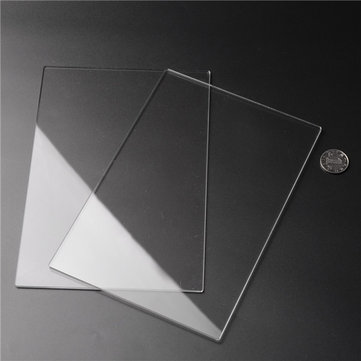
\includegraphics[width=1\textwidth]{figures/akrilik.jpg}
\caption{Bentuk Akrilik}
\label{print}
\end{figure}
\par Pada pembuatan rangka \textit{prototype} ini menggunakan akrilik. Akrilik adalah semacam plastik yang menyerupai kaca, namun memiliki sifat yang membuatnya lebih unggul daripada kaca, akrilik itu lembaran plastik yang super keras. Warnanya yang tak cepat pudar dan bobotnya yang ringan menjadi keunggulan akrilik hingga menjadi bahan baku barang kerajinan. Akrilik digunakan untuk membuat berbagai produk.  krilik adalah bagian dari plastik sintesis yang berasa dari asam akrilik, akrilik terbuat dari 100 MMA (metil metakrilat monomer), sudah paham kan temen-temen yuk kita bahas lebih dalam lagi mengenai akrilik. Akrilik memiliki nilai estetika yang tinggi selain tidak mudah pecah dan tahan cuaca, akrilik juga tidak akan berkerut atau mengembang, Akrilik lebih kuat dari kaca, sehingga lebih tahan dan tidak pecah sehingga lebih lebih aman.

\item \textbf{ Kabel Jumper}
\begin{figure}[H]
\centering
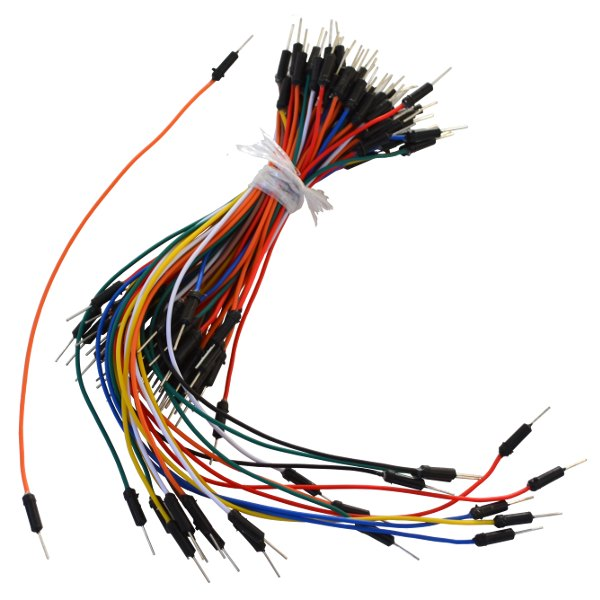
\includegraphics[width=1\textwidth]{figures/kabel.jpg}
\caption{Kabel Jumper}
\label{print}
\end{figure}

\par Kabel Jumper digunakan untuk menghubungkan komponen satu dengan komponen lainya. Selain itu kabel jumper ini juga untuk menghubungkan komponen dengan \textit{microcontroller}. Ada beberapa jenis kabel jumper yaitu sebagai berikut :


\begin{figure}[H]
\centering
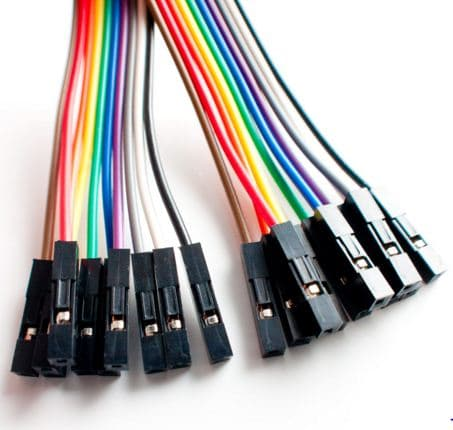
\includegraphics[width=1\textwidth]{figures/famel.jpg}
\caption{Kabel Jumper Famale}
\label{print}
\end{figure}

\begin{figure}[H]
\centering
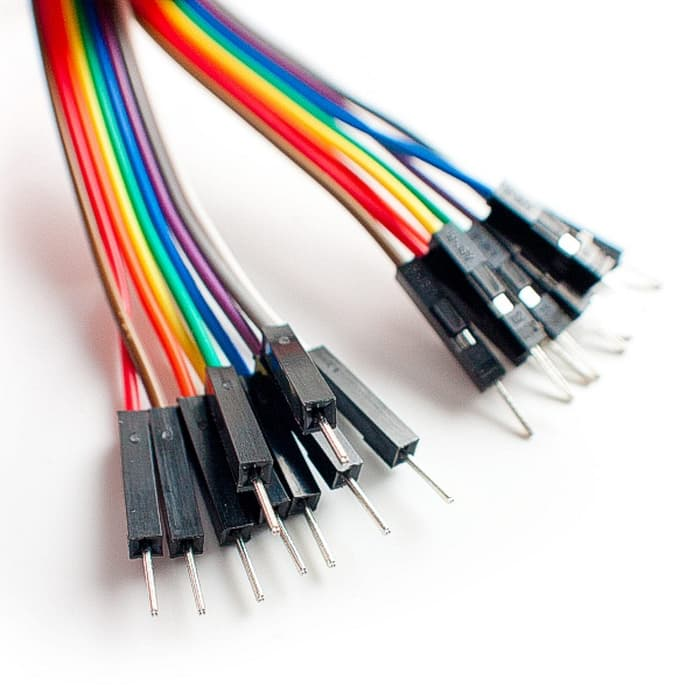
\includegraphics[width=1\textwidth]{figures/male.jpg}
\caption{Kabel Jumper Male}
\label{print}
\end{figure}

\begin{figure}[H]
\centering
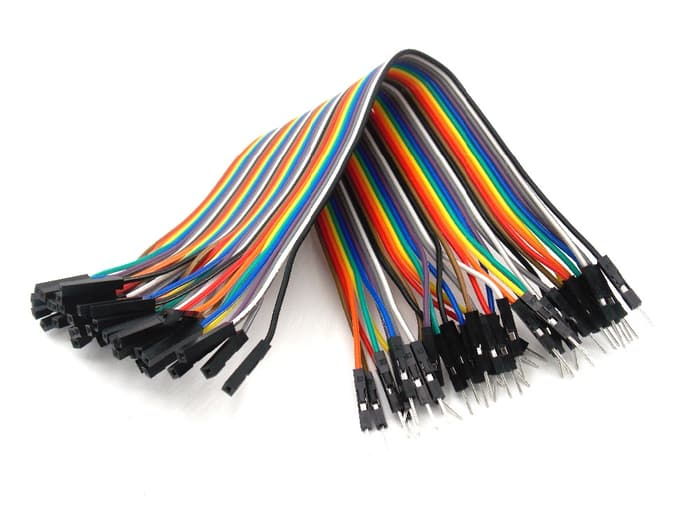
\includegraphics[width=1\textwidth]{figures/malefamale.jpg}
\caption{Kabel Jumper Male-Famale}
\label{print}
\end{figure}

\item \textbf{BreadBoard}
\par Breadboard adalah board yang digunakan untuk membuat rangkaian elektronik sementara dengan tujuan uji coba atau prototipe tanpa harus menyolder. Dengan memanfaatkan breadboard, komponen-komponen elektronik yang dipakai tidak akan rusak dan dapat digunakan kembali untuk membuat rangkaian yang lain. Breadboard umumnya terbuat dari plastik dengan banyak lubang-lubang diatasnya. Lubang-lubang pada breadboard diatur sedemikian rupa membentuk pola sesuai dengan pola jaringan koneksi di dalamnya.

\par Breadboard yang tersedia di pasaran umumnya terbagi atas 3 ukuran: mini breadboard, medium breadboard atau large breadboard. Mini breadboard memiliki 170 titik koneksi (bisa juga lebih). Kemudian medium breaboard memiliki 400 titik koneksi. Dan large breadboard memiliki 830 titik koneksi.

\begin{figure}[H]
\centering
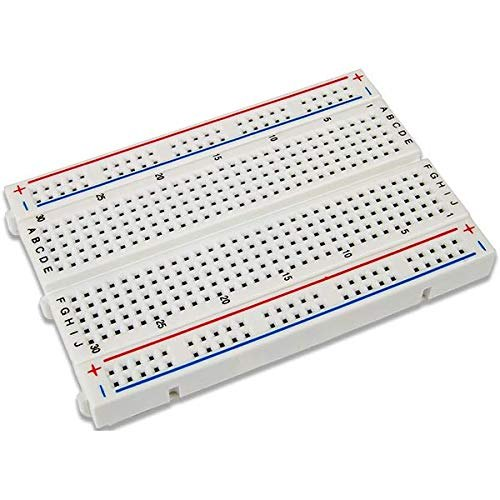
\includegraphics[width=1\textwidth]{figures/breadboard.jpg}
\caption{Breadboard Mini}
\label{print}
\end{figure}

\begin{figure}[H]
\centering
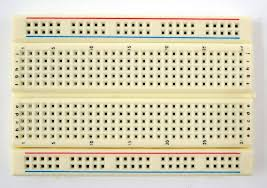
\includegraphics[width=1\textwidth]{figures/breadboard2.jpg}
\caption{Breadboard Medium}
\label{print}
\end{figure}

\begin{figure}[H]
\centering
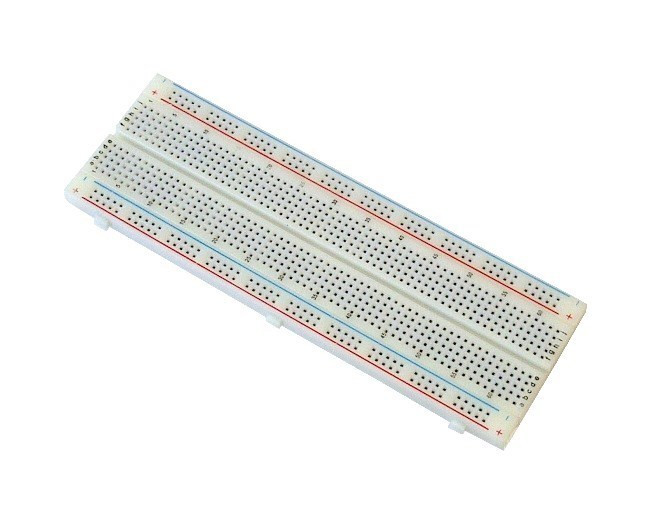
\includegraphics[width=1\textwidth]{figures/3.jpg}
\caption{Breadbroad Large}
\label{print}
\end{figure}


\end{enumerate}

\section{Pembuatan \textit{Prototype}}
Setelah membahas tentang komponen yang akan digunakan kemudian kita lanjutkan pada tahapan pembuatan \textit{prototype}. Dalam tahapan pembuatan \textit{prototype} ini tidak boleh ada salah satu step yang terlewatkan karena akan terjadi hal yang fatall. Berikut merupakan langkah-langkah pembuatan :
\begin{enumerate}
    \item Siapkan 6 buah akrilik bening berbentuk persegi empat berukuran 20cm x 20cm dengan ketabalan 3mm. Dengan memilih akrilik dengan ketebalan 3mm rangka pada \textit{prototype} yang akan dibuat akan lebih kuat dan lebih kokoh. Seperti pada gambar dibawah ini :
\begin{figure}[H]
\centering
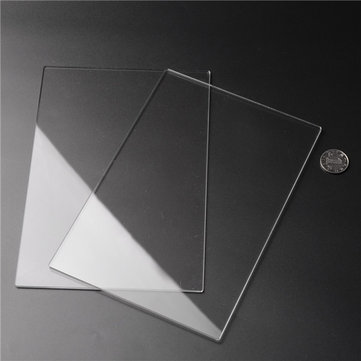
\includegraphics[width=1\textwidth]{figures/akrilik.jpg}
\caption{Contoh Akrilik yang digunakan}
\label{print}
\end{figure}

\item Siap lem korea atau lem akrilik untuk menempelkan akrilik satu dengan akrilik yang lainnya. Contoh lem yang harus digunakan sebagai berikut :

\begin{figure}[H]
\centering
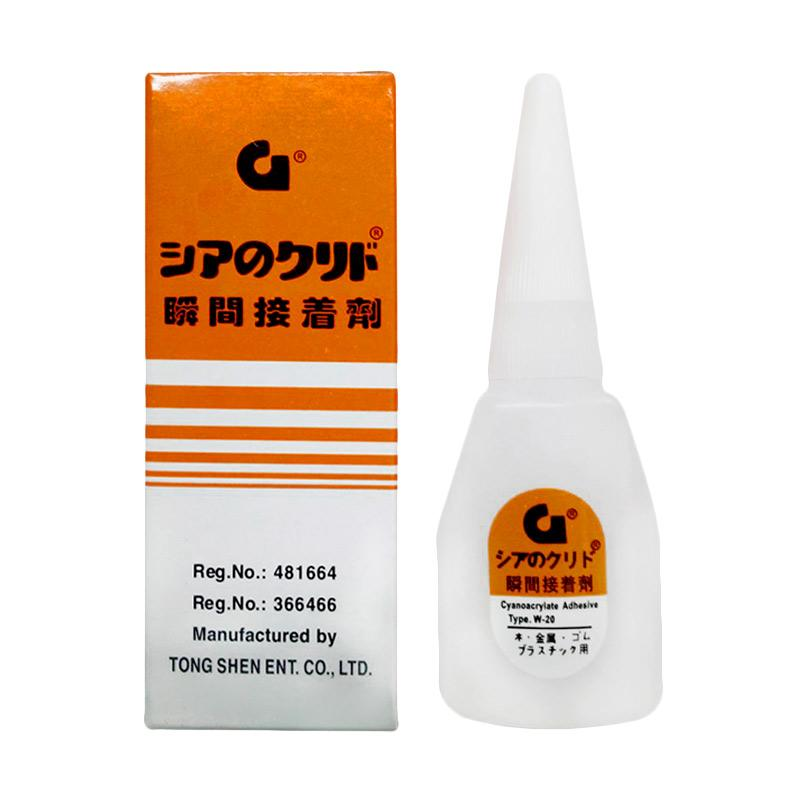
\includegraphics[width=1\textwidth]{figures/lem.jpg}
\caption{Contoh Lem Korea}
\label{print}
\end{figure}

\begin{figure}[H]
\centering
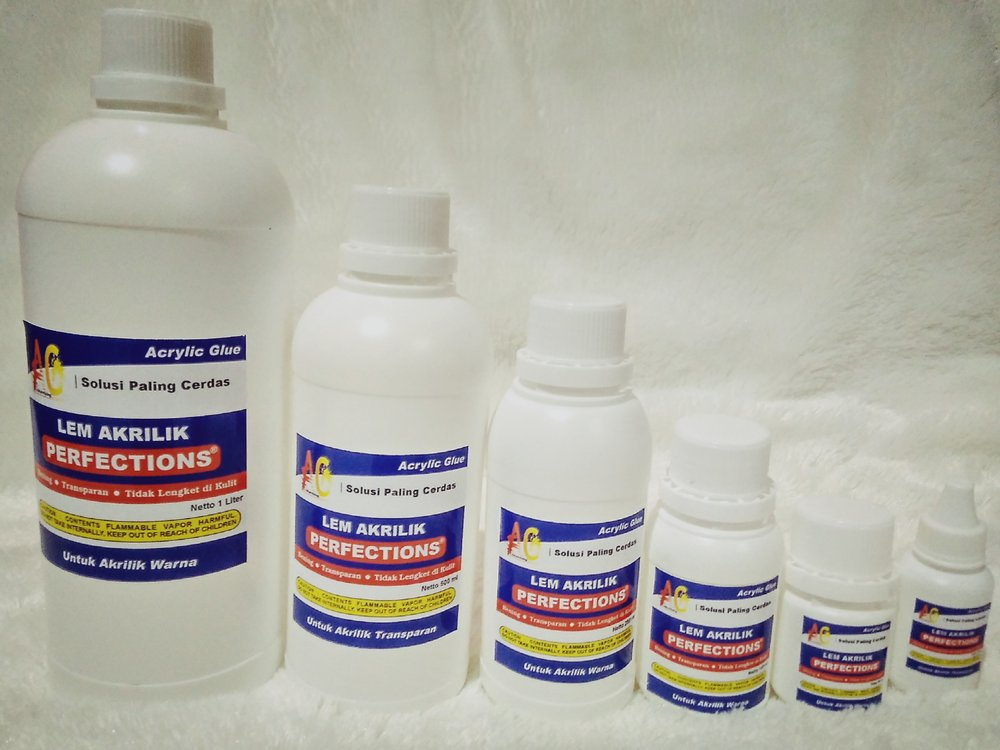
\includegraphics[width=1\textwidth]{figures/lem3.jpg}
\caption{Contoh Lem Akrilik}
\label{print}
\end{figure}

\par Pada pembuatan \textit{prototype} prediksi ketinggian air (PKA) untuk mendeteksi banjir sebagai peringatan dini ini menggunakan lem khusus akrilik, jikalau teman-teman ingin menggunakan lem korea tentunya bisa saja.Tetapi untuk masing-masing lem itu ada kelebihan maupun kekuranganya. 

\par Kenapa saya lebih memilih lem akrilik dibandingkan lem korea? karena lem akrilik lebih kuat untuk menempalkan akrilik satu dengan akrilik lainnya, hanya dengan sekali olesan. Sedangkan lem korea agar lebih kuat menempelkan akrilik satu dengan yang lainya harus mengoleskan lemnya beberapa kali. Selain itu jika mengguanakan lem korea teksturnya sangat cair sehingga lem akan berceceran yang mengakibatkan tidak rapih pada saat proses menempelkan akrilik.

\par Selain hal tersebut ada beberapa faktor lagi yaitu  jika mengunakan lem akrilik kita tidak perlu membutuhkan lem terlalu banyak karna hanya perlu satu olesan saja untuk merekatkan akrilik seperti yang telah dijelaskan sebelumnya. Sebalik nya jika kita menggunakan lem korea maka kita membutuhkanlem korea yang lebih banyak dibandingkan dengan lem akrilik. 

\par Disamping hal itu jika kita menggunkan lem akrilik ada kekurangannya juga dalam segi \textit{cost} atau pengeluaran dikarenakan lem akrilik lebih mahal dibandingkan dengan lem korea.


\item Siapkan sticky note warna warni. Sticky note ini akan digunakan sebagai level peringatan pada kerangka \textit{prototype}. Contoh sticky note yang digunakan sebagai berikut :
\begin{figure}[H]
\centering
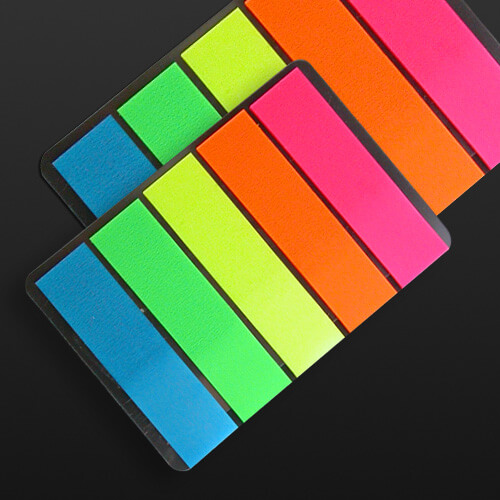
\includegraphics[width=1\textwidth]{figures/note.jpg}
\caption{Contoh Sticky Note}
\label{print}
\end{figure}

\par Warna Sticky note yang digunakan hanya 3 warna tidak akan menggunakan semua warna. Warna yang digunkan yaitu warna merah, hija, dan kuning. Warna merah digunakan untuk level awas banjir, warna hijau digunakan untuk level siaga banjir dan warna kuning digunakan untuk level aman dari banjir.

\par Jika teman-teman ingin mengganti warna-warna sticky note untuk level-level banjir tentu saja boleh . Tapi harus ada beberapa hal yang harus diperhatikan karena setiap warna memiliki arti atau \textit{filosofi}nya yang berbeda. Seperti contohnya teman-teman memilih warna coklat untuk level awas banjir itu sangat tidak \textit{sinkron}.

\item Siapkan double tape, karena double tape inu akan dugunakan untuk menepelkan sticky note pada kerangka \textit{prototype}.

\begin{figure}[H]
\centering
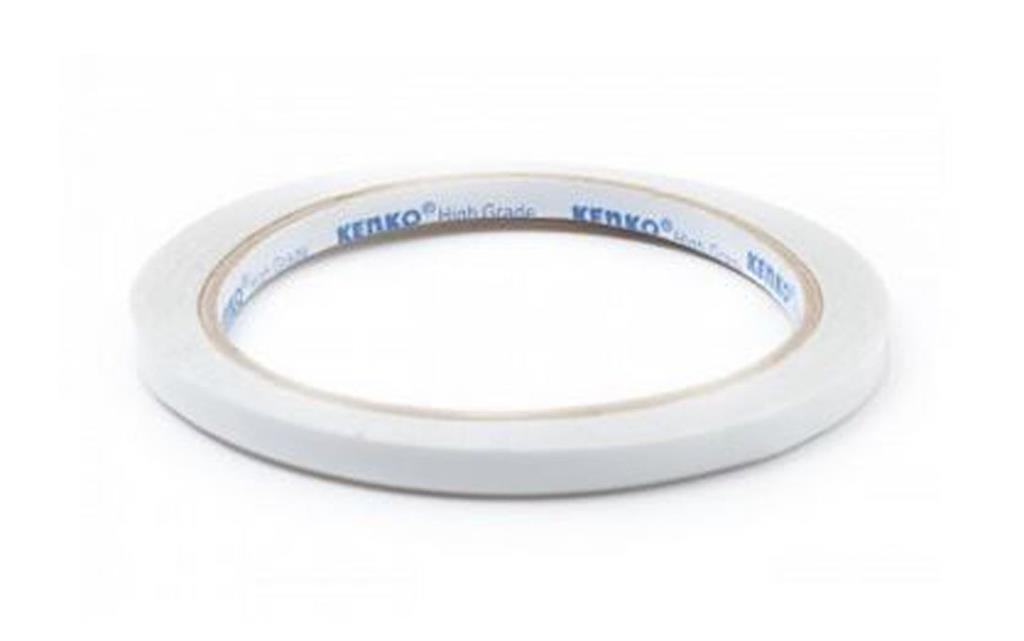
\includegraphics[width=1\textwidth]{figures/double.jpg}
\caption{Contoh Double TApe}
\label{print}
\end{figure}

\par Disini menggunakan double tape dengan ukuran yang kecil karena disesuaikan dengan ukuran sticky note yang digunakan. Jika teman-teman menggunakan sticky note yang berukuran sedang maka harus menggunakan double tape yang berukuran sedang agar sticky note dapat menempel dengan rapih.

\item \textbf{\textit{styrofoam} papan}
\begin{figure}[H]
\centering
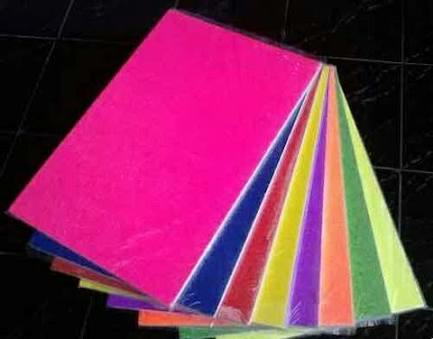
\includegraphics[width=1\textwidth]{figures/sterofoam.png}
\caption{Contoh Styrofoam Papan}
\label{print}
\end{figure}

\par \textit{styrofoam} papan ini digunakan untuk alas komponen pada kerangka \textit{prototype} prediksi ketinggian air (PKA) untuk mendeteksi banjir peringatan dini. Fungsi diberikan alas untuk komponen yaitu agar komponen tidak bersentuhan langsung dengan permukaan akrilik.

\end{enumerate}

\section{Merakit \textit{Kerangka Prototype}}
\par Setelah semua komponen dan bahan- bahan yang dibutuhkan untuk membuat prototipe ini tersedia. Maka tahapan selajutnya yaitu perakitan alat.perhatikan langkah- langkah berikut ini :
\begin{enumerate}
    \item Tempelkan akrilik menjadi berbentuk seperti kubus, tetapi pada bagian atas atau atap nya tidak perlu ditutup sehingga seperti pada gambar dibawah ini : 
    

\begin{figure}[H]
\centering
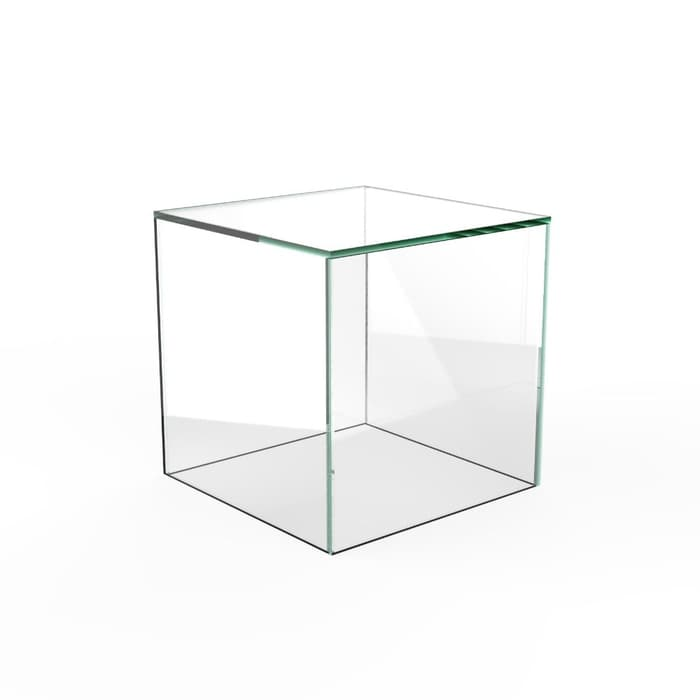
\includegraphics[width=1\textwidth]{figures/kubus.jpg}
\caption{Kerangka Prototipe}
\label{print}
\end{figure}

\item Setelah itu membuat kotak kotak kecil yang nantinya sebagai tempat komponen. Sehingga seperti gambar dibawah ini :


\begin{figure}[H]
\centering
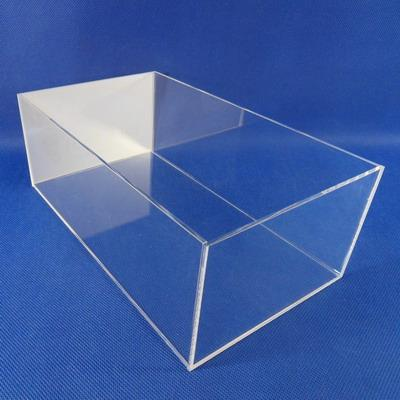
\includegraphics[width=1\textwidth]{figures/kubus2.jpg}
\caption{Kerangka Prototipe Tempan Penyimpanan Komponen }
\label{print}
\end{figure}

\par Setalah kedua rangka prototipe tersebut dibuat maka rekatkan kerangka tersebut dengan kerangka prototipe yang sebelumnya yang telah dibuat. Caa merekatkanya yaitu dengan lem korea atau lem akrilik sesuai dengan pembahasan sebelumnya.

\end{enumerate}

\section{Perakitan dan Memprogram Komponen \textit{Prototype}}
\subsection{Perakitan Komponen}

\par Komponen elektronika adalah komponen yang paling kompleks dan sensitif, tak jarang terjadi kerusakan apabila komponen yang digunakan tak seuai semestinya, misalkan kelebihan daya, arus, short, dll. Selain itu tidak semua komponen ataupun perangkat elektronika dapat dijumpai dan dibeli dengan mudah, salah satu contohnya adalah osiloskop, spektrum analizer, function generator, dll.

\par Maka dari itu software simulasi dapat membatu proses merancang rangkaian elektronika sebelum dipatenkan langsung pada komponen. Bukan hanya itu, kitapun dapat menggunakan perangkat elektronika yang tidak dapat kita jangkau (beli dan dijumpai) seperti halnya osiloskop dalam software simulasi tersebut.
\par Untuk membuat suatu rangkaian atau skema kita bisa menggunakan beberapa software seperti :
\begin{enumerate}
    \item Frizting
    \par Fritzing merupakan aplikasi berbasis free software yang dapat kita unduh secara gratis. Aplikasi ini berfungsi untuk membuat sebuah skema rangkaian elektronika secara nyata (real) Karena komponen yang berada pada rangkaian tersebut digambarkan dengan sangat mirip dengan komponen aslinya. Aplikasi ini tidak hanya dilengkapi dengan skema rangkaian yang sangat baik, banyak fitur lainnya yang dapat kita coba seperti PCB layout dan programming Arduino langsung pada aplikasi ini. Sayangnya aplikasi ini hanya dapat membuat skema saja, kita tidak dapat melakukan simulasi pada rangkaian yang sudah kita buat.
\begin{figure}[H]
\centering
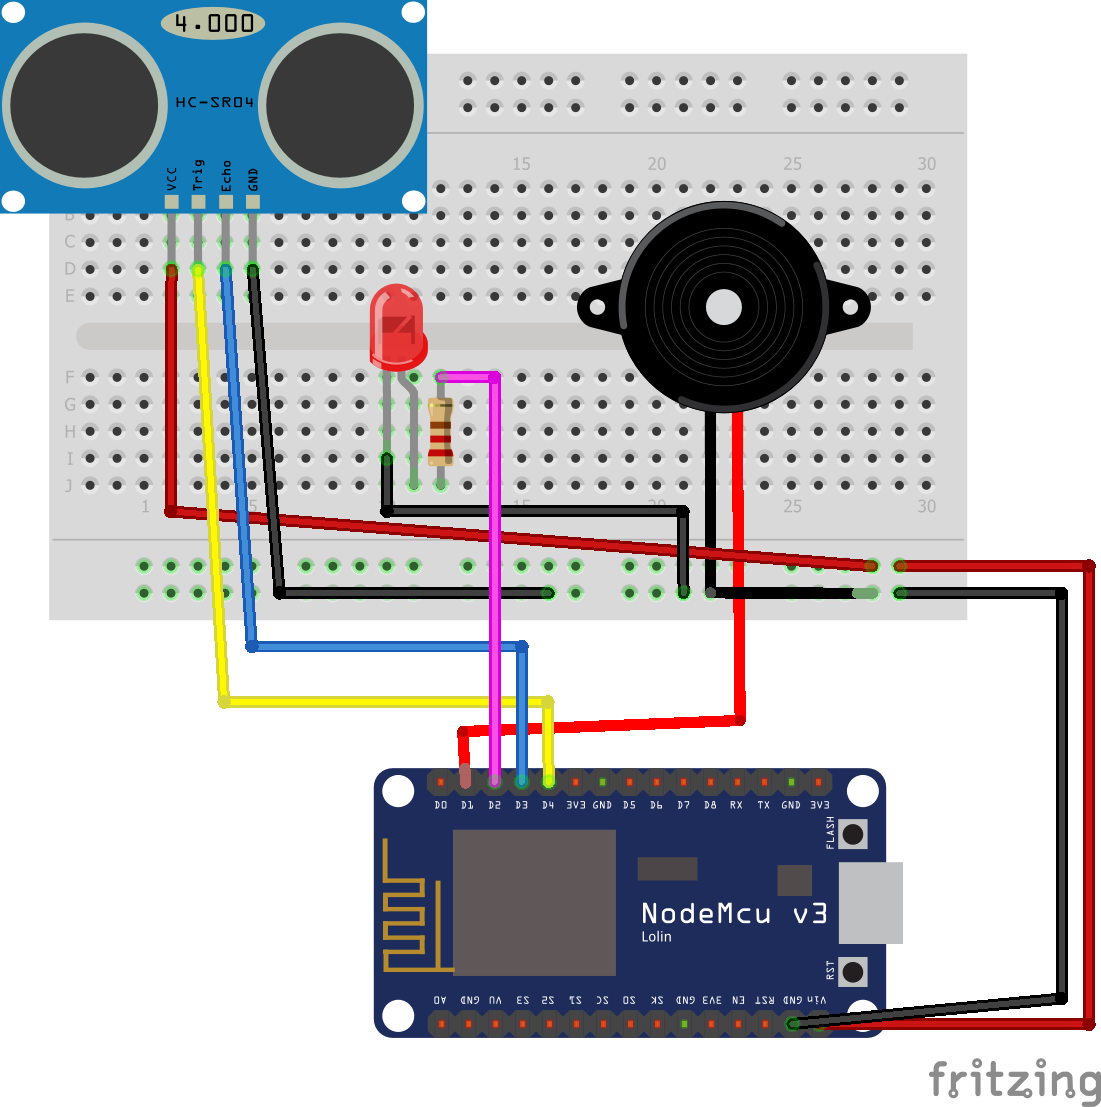
\includegraphics[width=1\textwidth]{figures/rangkaian.png}
\caption{Rangkaian Alat  }
\label{print}
\end{figure}
    
    
    \item LiveWire
    \item Electronics Workbench (EWB)
    \item NI Multisim
    \item Autodesk Circuits
    \item Proteus ISIS
\end{enumerate}


\par Tahapan selanjutnya yaitu membuat atau merakit komponen untuk prototipe. Tetapi ada satu hal sebelum kita masuk ke proses perakitan yaitu kita harus membuat sebuah rangkaian atau skema komponen. Tujuan dibuatnya suatu rangkaian atau skema ini untuk mempermudah kita pada saat proses perakitan. 

perhatikan  langkah - langkah berikut ini :
\begin{figure}[H]
\centering
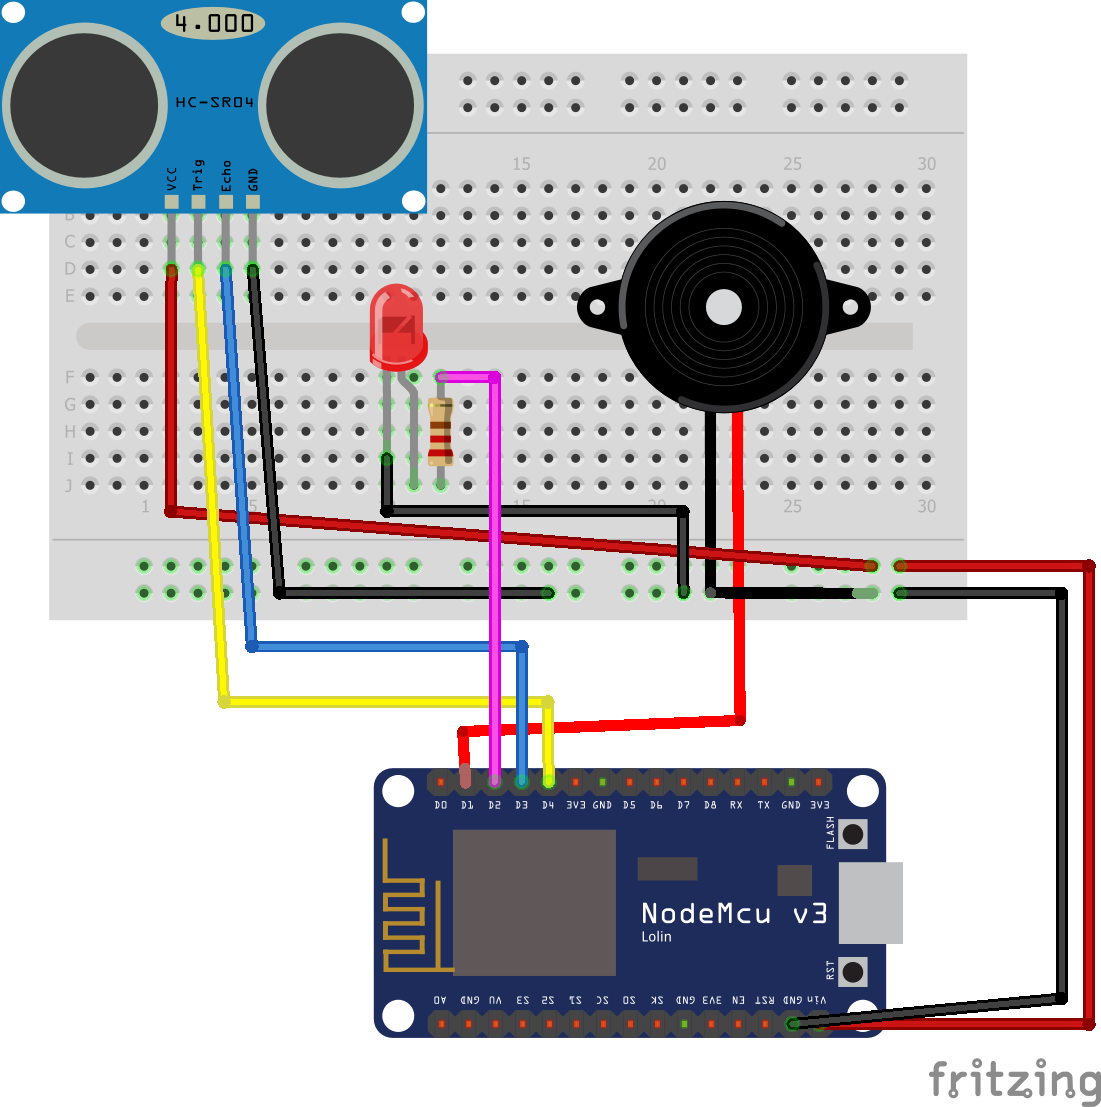
\includegraphics[width=1\textwidth]{figures/rangkaian.png}
\caption{Rangkaian Alat  }
\label{print}
\end{figure}

\par Agar mempermudah  pada saat proses perakitan komponen maka harus mengikuti gambar rangkaian diatas. Untuk penjelasannya sebagai berikut :
\begin{enumerate}
    \item Sambungkan Vin pada NodeMCU pada \textit{breadboard} bagian positif (+). Vin merupakan Power atau VCC dengan memiliki daya 5V. Jadi jika tidak ada 5V dalam sebuah \textit{microcontroller} dapat di gantikan dengan vin.
\end{enumerate}

